\documentclass[12pt]{article}
\usepackage{natbib}
\usepackage[english, french]{babel}
\usepackage[utf8]{inputenc}
\usepackage[T1]{fontenc}
\usepackage{tikz}
\usepackage{amsmath}
\usepackage{textcomp}
\usepackage{graphics}
\usepackage{graphicx}
\usepackage{multirow}
\usepackage{url}
\usepackage{psfrag}
\usepackage{fancyhdr}
\usepackage{vmargin}
%\usepackage[backend=biber]{biblatex}
\usepackage{csquotes}
\usepackage[hidelinks]{hyperref}
\usepackage{enumitem}
\usepackage[justification=centering]{caption}
\usepackage{array,multirow,graphicx}
\usepackage{float}
\usepackage{mathtools}
\usepackage{graphicx}
\usepackage{caption}
\usepackage{ifthen}
\usepackage{color}
\usepackage{xcolor}
\usepackage{listings}
%\usepackage{setspace}
%\usepackage{pdfpages}

%\def\rot#1{\rotatebox{90}{#1}}

\DeclarePairedDelimiter\ceil{\lceil}{\rceil}
\DeclarePairedDelimiter\floor{\lfloor}{\rfloor}

\setmarginsrb{1.5 cm}{1 cm}{1.5 cm}{1 cm}{0.51 cm}{1 cm}{0.5 cm}{1 cm}
\setlength{\parindent}{1cm}

\title{Application de gestion de données du Concours Mines-Télécom}
\author{Ahmed, Céline, Maël}
\date{Avril 2021}

\makeatletter
\let\thetitle\@title
  \let\theauthor\@author
\let\thedate\@date
\makeatother

\pagestyle{fancy}
\fancyhf{}
\rhead{\theauthor}
\lhead{\thetitle}
\cfoot{\thepage}

\begin{document}

\begin{titlepage}
    \centering
    
 	
\includegraphics[scale=0.36]{Images/logo/logo_TN_horizontal}\\[1.0 cm]
 	
	\textsc{\LARGE TELECOM Nancy}\\[1.5 cm]
	\textsc{\Large Rapport de Projet PII}\\[0.5 cm]
	%\textsc{\large code de l'UE}\\[0.5 cm]
	{\large \thedate}\\[0.5 cm]
	\rule{\linewidth}{0.2 mm} \\[0.5 cm]
	{ \huge \bfseries \thetitle}\\[0.2 cm]
	\rule{\linewidth}{0.2 mm} \\[1.5 cm]
	\textsc{\large Groupe 9}\\[1.0 cm]
	
	\begin{minipage}{0.4\textwidth}
		\begin{flushleft} \large
		\emph{Étudiants:}\\
			Maël SAILLOT \\
			Céline ZHANG \\
			Ahmed ZIANI
		\end{flushleft}
	\end{minipage}~
	\begin{minipage}{0.4\textwidth}
		\begin{flushright} \large
		\emph{Numéro Étudiant:}\\
			31831300 \\
			32024925 \\
			31824316
		\end{flushright}
	\end{minipage}\\[1.4 cm]
	
	\large
	\emph{Encadrants du projet :}\\
	   Sébastien DA SILVA\\
	   Gérald OSTER\\
	   ~ \\
	   ~ \\[1.5 cm]

	
\includegraphics[scale=0.12]{Images/logo/logo_UL_horizontal}\\[1 cm]

	\vfill
\end{titlepage}

\newpage
%%%%% Remerciements %%%%%
\section*{\center Remerciements}

\hskip7mm

%\begin{spacing}{}
Nous tenons à remercier chaque membre de l'équipe pour leurs contributions à la réalisation de ce projet ainsi que toute l’équipe pédagogique  de Telecom Nancy, en particulier à M. Gérald OSTER, M. Sébastien DA SILVA et M. Christophe BOUTHIER, pour l’aide qu’ils nous ont apporté afin de mener à bien notre scolarité durant ces temps difficiles, et tout au long du projet. \\
%\end{spacing}

\newpage

%%%%% Résumé %%%%%
\begin{abstract}
   % \renewcommand{\abstractname}{Résumé}
% résumé du projet en français
Le projet concerne une application de gestion de la base de données du concours Mines-Télécom. Cette application doit être facile à utiliser, elle doit permettre à l'utilisateur d'accéder aux informations des candidats simplement, et d'afficher des résultats (notes, rangs, écoles, coordonnées, bac, etc.), ils doivent pouvoir être filtré si nécessaire. Afin de réaliser une tel application, le groupe a commencé la création d'un modèle adapté aux données fournies, puis a rempli la base de données issue de ce modèle. Ensuite, elle a fait l'implémentation de l'application et des fonctionnalités (affichage, filtrage, recherche, etc). Par ailleurs, la cohérence des données doit être vérifiée, en conséquence, un script de vérification a été réalisé.
\end{abstract}

\renewcommand{\abstractname}{Abstract}

\begin{abstract}
% résumé du projet en anglais
This project is about an application that will help manage the Mines-Télécom competitive exam data. The application needs to be easy to use, the user should be able to access easily to candidates information, and it needs to display the results (scores, ranks, schools, contact information, graduation, etc.) that have to be filtered when necessary. In order to create this app, the team started by visualizing it through a model that was in compliance with the given datas, before filling the database with the model. Then, the team implemented the app and its features (display, filtering, search, etc). Besides, the data’s consistency needs to be checked, that is the reason why a test script was written.
\end{abstract}

\newpage

\tableofcontents

\newpage

%%%%% Introduction %%%%%
\section*{Introduction} 
    \addcontentsline{toc}{section}{Introduction}
    % A relire
    
Dans le cadre de notre module PPII, il est demandé de faire un projet mettant oeuvre à la fois nos compétences en base de données relationnelles, nos compétences en programmation de script, et nos connaissances en web. Le projet a pour finalité le développement d'une application qui permet la gestion d'une base de données du concours Mines-Télécom. \\
    
    L'objectif de ce projet est de réaliser une structure de base de données relationnelles respectant les critères de la troisième forme normale à partir des informations fournies par l'utilisateur. Les informations concernent les candidats inscrits aux concours d'admission des écoles de la banque Mines-Télécom, elles doivent être mises dans la base de données relationnelles produite. L'application demandée doit pouvoir accéder aux informations de la base de données et les afficher de plusieurs manières. Un script de test de cohérence des données est nécessaire pour omettre toute erreur dans nos données. La performance est demandée, le remplissage des tables de la base de données par le script ne doit pas dépasser une certaine durée précisée dans le cahier des charges.\\
    
    Tout d'abord, nous devons créer notre base de données, c'est-à-dire réaliser notre modèle de données relationnelles respectant la troisième forme normale et les contraintes de certains champs. Ensuite, il faut remplir les tables de la base de données par les données fournies, de ce fait des fonctions d'importation de données, regroupées dans un script de remplissage, ont été implémentées. Puis, une vérification des tables a été faite pour identifier les données manquantes, les erreurs de remplissage, et les données inutilisables (comme les candidats anonymes). Enfin, pour afficher ces données par un utilisateur, nous avons lis en place une application web qui permet de montrer les données de plusieurs manières selon les demandes. Les principales technologies utilisées sont \textsf{SQLite3} qui permet de créer la base de données, \textsf{SQLiteStudio} qui permet d'afficher la base de données, les bibliothèques \textsf{Flask}, \textsf{Pandas}, \textsf{Openpyxl} de \textsf{Python} pour écrire les scripts et l'application web.\\
    
    Les résultats du projet sont présentés dans ce rapport, il y a une partie consacrée à l'état de l'art, c'est-à-dire la présentation des notions en base de données relationnelles, et l'explication théorique des procédés utilisés~; une partie consacrée à l'implémentation et l'application de l'algorithme, elle explique le raisonnement entre les lignes de codes, et présente les résultats lors de l'exécution des codes. Dans ce rapport se trouve également une partie pour les tests et les performances des fonctions réalisées~; une partie présentant la gestion de projet de l'équipe et les moyens utilisés. À la fin de ce rapport, se trouvent les annexes, dans lesquelles se rangent les déclarations de non-plagiat, les tableaux d'organisation du travail, les comptes rendus de réunions, et d'autres divers documents.
    % Elles sont rangés dans des tableaux numérique (fichiers \texttt{.xlsx}, \texttt{.csv}) avec des champs indiquant la nature de ces informations. 

\newpage

    \subsection*{Cahier des charges}
        \addcontentsline{toc}{subsection}{Cachier de charges}
    \begin{table}[h]
        \centering
        \begin{tabular}{|l|}
            \hline
            \textbf{Travaux demandés}  \\
            \hline
            Base de données pour les informations du concours des Mines-Télécom \\
            Script de remplissage de la base de données \\
            Temps de remplissage < 3 min \\
            Application permettant d'accéder aux données (candidats, notes, classements, diverses) \\
            Affichage des résultats de recherches dans l'application avec des graphes ou sur une carte \\
            Amélioration de l'apparence de l'application \\
            Faciliter l'utilisation de l'application (rendre interactif) \\
            Tests de cohérence des données fournies et du remplissage \\
            % Calcul de complexité \\
            % Mesures de performances des fonctions \\
            \hline
        \end{tabular}
        \caption{Le cahier des charges}
        \label{tab:cdc}
    \end{table}

    \subsection*{Mentions légales}
        \addcontentsline{toc}{subsection}{Mentions légales}
        
    Ce projet n’est pas destiné à un usage commercial, ainsi, les images présentés, notamment les images de tests, d'applications ou de gestion de projet, ne sont pas destinées à la publication. \\
    Cependant, le caractère strictement scolaire de ce projet nous autorise à les inclure en accord avec :
    \begin{itemize}%[label=\textbullet]
    \item Code civil : articles 7 à 15, article 9 : respect de la vie privée
    \item Code pénal : articles 226-1 à 226-7 : atteinte à la vie privée
    \item Code de procédure civil : articles 484 à 492-1 : procédure de référé
    \item Loi n78-17 du 6 janvier 1978 : Informatique et libertés, Article 38
    \end{itemize}
    Les déclarations sur l’honneur de non-plagiat des membres de l’équipe du projet sont présentés dans les quatre premières pages de l'annexe.

    Cette version\footnote{version 1} du rapport a été finalisée le 11 Juin 2021.

\newpage

%%%%% État de l'art %%%%%
\section{État de l'art}
    % A relire
    Actuellement, nous sommes dans un monde qui exploite fortement des données, que ce soit pour l'administration, l'économie ou le divertissement. Un problème de gestion de ces données se pose, notamment les limites de stockage et le temps d'accès aux données. Il existe de nos jours plusieurs manières gérer ces données de manière optimale, ce sont les structures de base de données relationnelles. Pour qualifié la robustesse d'un modèle relationnel, nous avons plusieurs critères à vérifier. Ces critères ainsi que notre modèle sont présentés dans les paragraphes suivants. 
    %%% parler des clés primaires, étrangères et des contraintes.
    \subsection{Formes normales}
        % A relire
        Les formes normales sont les résultats de la normalisation des modèles de données permettant, selon le niveau, d'éviter les redondances, les problèmes de mise à jour, de garder la cohérence et d'optimiser le stockage des données. Dans le modèle de type OLTP\footnote{online transaction processing, en français, le traitement transactionnel en ligne est un type d'application informatique qui sert à effectuer des modifications d'informations en temps réel.~\cite{oltp}}, il existe huit formes normales. Les trois premières sont les plus connus, c'est ce que nous allons rappeler~\cite{fn}. Le non-respect de ces règles engendre des redondances inutiles. Dans les exemples qui suivent, les attributs soulignés forment les clés.
        \subsubsection{Première forme normale}
            % Parler du blabla de la forme normale.
            Une relation (ayant par définition une clé) dont les attributs possèdent tous une valeur sémantiquement atomique\footnote{ce qu'on ne peut pas diviser.}. Les attributs constitués par un ensemble de valeurs énumérées dont les différentes valeurs sont sémantiquement indépendantes et les attributs n'ayant aucune valeur violent l'atomicité. 
            \begin{figure}[!h]
                \centering
                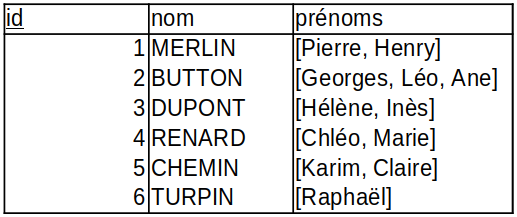
\includegraphics[scale = 0.5]{Images/Etat de l'art/non_atomique.png}
                \caption{Exemple de table non-atomique, l'attribut \texttt{prénoms} viole l'atomicité}
                \label{fig:non-atomique}
            \end{figure}
            % \begin{table} [!h]
            %     \begin{center}
            %     \begin{tabular}{|l|l|l|}
            %     \hline
            %       & & \\
            %     S & & \\
            %     M & & \\
            %     A & & \\
            %     R & & \\
            %     T & & \\
            %     \hline
            %     \end{tabular}
            %     \end{center}
            %     \caption{La méthode SMART}
            %     \label{tab:SMART}
            % \end{table}
            
        \subsubsection{Deuxième forme normale}
            Les attributs d’une relation sont séparés en deux groupes, le premier est composé de la clé, qui peut être un ou plusieurs attributs, et le deuxième est composé des autres attributs, éventuellement vide. Pour respecter la 2FN\footnote{deuxième forme normale}, il faut d'abord respecter la 1FN, et il faut que tout attribut du deuxième groupe ne dépende pas d’un sous-ensemble (strict) d’attribut(s) du premier groupe. C'est-à-dire, un attribut non clé ne dépend pas d’une partie de la clé mais de toute la clé~\footnote{extrait de~\href{https://fr.wikipedia.org/wiki/Forme\_normale\_(bases\_de\_données\_relationnelles)}{\textsf{Wikipédia 2FN}}}.
            \begin{figure}[!h]
                \centering
                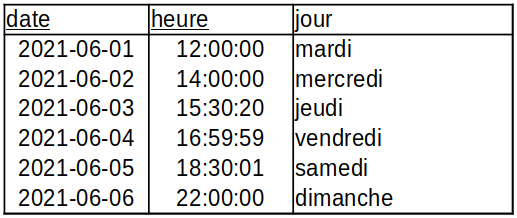
\includegraphics[scale = 0.5]{Images/Etat de l'art/non-2FN.png}
                \caption{Exemple de table non-2FN, l'attribut \texttt{jour} ne dépend que de l'attribut \texttt{date}}
                \label{fig:non-2FN}
            \end{figure}
        
        \subsubsection{Troisème forme normale}
            Pour respecter la 3FN, il faut d'abord respecter la 2FN et il faut que tout attribut du deuxième groupe ne dépende pas d’un sous-ensemble (strict et excluant l’attribut considéré) d’autres attribut(s) du second groupe. C'est-à-dire, un attribut non clé ne dépend pas d’un ou plusieurs attributs ne participant pas à la clé. Autrement dit~: « Tous les attributs non clé doivent dépendre directement de la clé, au sens où il n’y a aucun attribut non clé dépendant de la clé par dépendances transitives par l’intermédiaire d’autres attributs non clé »~\footnote{extrait de~\href{https://fr.wikipedia.org/wiki/Forme\_normale\_(bases\_de\_données\_relationnelles)}{\textsf{Wikipédia 3FN}}}.
            \begin{figure}[!h]
                \centering
                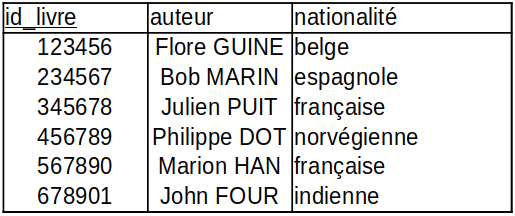
\includegraphics[scale = 0.5]{Images/Etat de l'art/non-3FN.png}
                \caption{Exemple de table non-3FN, l'attribut \texttt{nationalité} dépend de l'attribut \texttt{auteur}}
                \label{fig:non-3FN}
            \end{figure}
    
    \subsection{Conception de la structure}
    
    Nous avons en tout 18 tables contenant des champs dans lesquels on range les informations. Les tables sont représentées dans le modèle de données qui se trouve ci-après, Figure~\ref{fig:bd1}. L'outil \textsf{dbdiagram.io} a été utilisé pour faire la représentation graphique du modèle de données. Voici une présentation des tables conçues~:
        \begin{itemize}[label=\textbullet]
            \item \textbf{candidat}~: affiche les informations du candidat inscrit sur le site \textsf{scei}, la clé primaire est le numéro unique du candidat~;
            \item \textbf{classe}~: stock les différentes classes associées à une clé primaire~, utile pour remplir le champ \texttt{classe} de la table \texttt{candidat} représentant la classe d'origine, en relation \texttt{1N} (\textsl{foreign key})~;
            \item \textbf{civilite}~: sauvegarde les appellations, Monsieur ou Madame (il est possible d'en ajouter), chacun identifié à une clé primaire, cela permet de gagner du stockage sur l'attribut \texttt{civ} de la table \texttt{candidat}, en relation \texttt{1N}~;
            \item \textbf{ep\_option}~: regroupe les différentes combinaisons pour les épreuves d'options (par exemple LV1 Espagnol), elles sont associées par clé primaire, cette table permet de remplir les champs \texttt{option1}, \texttt{option2}, \texttt{option3}, \texttt{option4} de la table \texttt{candidat}, en relation \texttt{1N}~;
            \item \textbf{etat\_dossier}~: on y trouve le code avancement du dossier du candidat, permet de remplir le champ \texttt{dossier} de la table \texttt{candidat}, en relation \texttt{1N}~;
            \item \textbf{serie\_bac}~: contient les différents BAC (S, ES, STI2D, etc.), permet de remplir le champ \texttt{bac} de la table \texttt{candidat}, en relation \texttt{1N}~;
            \item \textbf{csp\_parent}~: on y trouve les différents milieux socio-professionnel des parents, associé à une clé primaire~, utile pour remplir les champs \texttt{csp\_pere}, \texttt{csp\_mere} de la table candidat, en relation \texttt{1N}~;
            \item \textbf{pays}~: garde les différents pays et la nationalité correspondante sont associés à une clé primaire qui sert de \textsl{foreign key} pour la relation \texttt{1N} des champs \texttt{code\_adr\_pays}, \texttt{code\_pays\_naissance}, \texttt{code\_pays\_nationalite} de la table \texttt{candidat}~;
            \item \textbf{autres\_prenoms}~: 2e prénoms de certains candidats, lié à une \textsl{foreign key} (\texttt{candidat.code}-\texttt{1N}-\texttt{etudiant})~; 
            \item \textbf{epreuve}~: contient les différentes épreuves, ont un nom (\texttt{lib}) unique et un type, la clé primaire \texttt{epreuve.id} est une clé étrangère de ma table \texttt{notes}~; 
            \item \textbf{notes}~: stock les résultats des candidats selon les épreuves identifiées par leur \texttt{id} de la table \texttt{epreuve}~;
            \item \textbf{type\_classement}~: admissible, admis, etc., il est nécessaire de différencier les types de classements pour savoir à quoi correspondant le classement demandé, la clé primaire de cette table s'utilise en clé étrangère dans la table \texttt{classement}~;
            \item \textbf{classement}~: on a besoin d'identifier la nature du classement, d'où la \texttt{FK}\footnote{foreign key} en champ \texttt{type}, la clé primaire indique le classement unique, et on demande aussi à que \texttt{etudiant} (en \texttt{FK} avec \texttt{candidat.code}, relation \texttt{1N}) et \texttt{type} soient un couple unique~; 
            \item \textbf{ecole}~: rassemble les écoles, le \texttt{lib} est associé à une clé primaire qui sert de clé étrangère à \texttt{voeux.ecole}~; 
            \item \textbf{voeux}~: regroupe les voeux émis des candidats, la table est composée d'une clé primaire \texttt{code}, d'une clé étrangère qui vient de \texttt{ecole.code}, et d'un ordre de classement~;
            \item \textbf{concours}~: contient les différentes filières du concours, avec \texttt{lib}\footnote{nom du concours} et \texttt{voie}\footnote{la voie du concours}, le champ \texttt{concours.code} est la clé primaire qui sert de clé étrangère à \texttt{candidat.voie\_concours} en relation \texttt{1N}~;
            \item \textbf{etablissement}~: regroupe tous les établissements d'origine des candidats, \texttt{rne} est la clé primaire qui sert de \texttt{FK} pour \texttt{candidat.etablissement}, suivi des attributs donnant des informations sur l'établissement~;
            \item \textbf{etat\_reponse}~: on y trouve les différents états de réponse (lors de la phase admission certainement), c'est la seule table qui est reliée à rien.
        \end{itemize}
            \begin{figure}[!h]
                \centering
                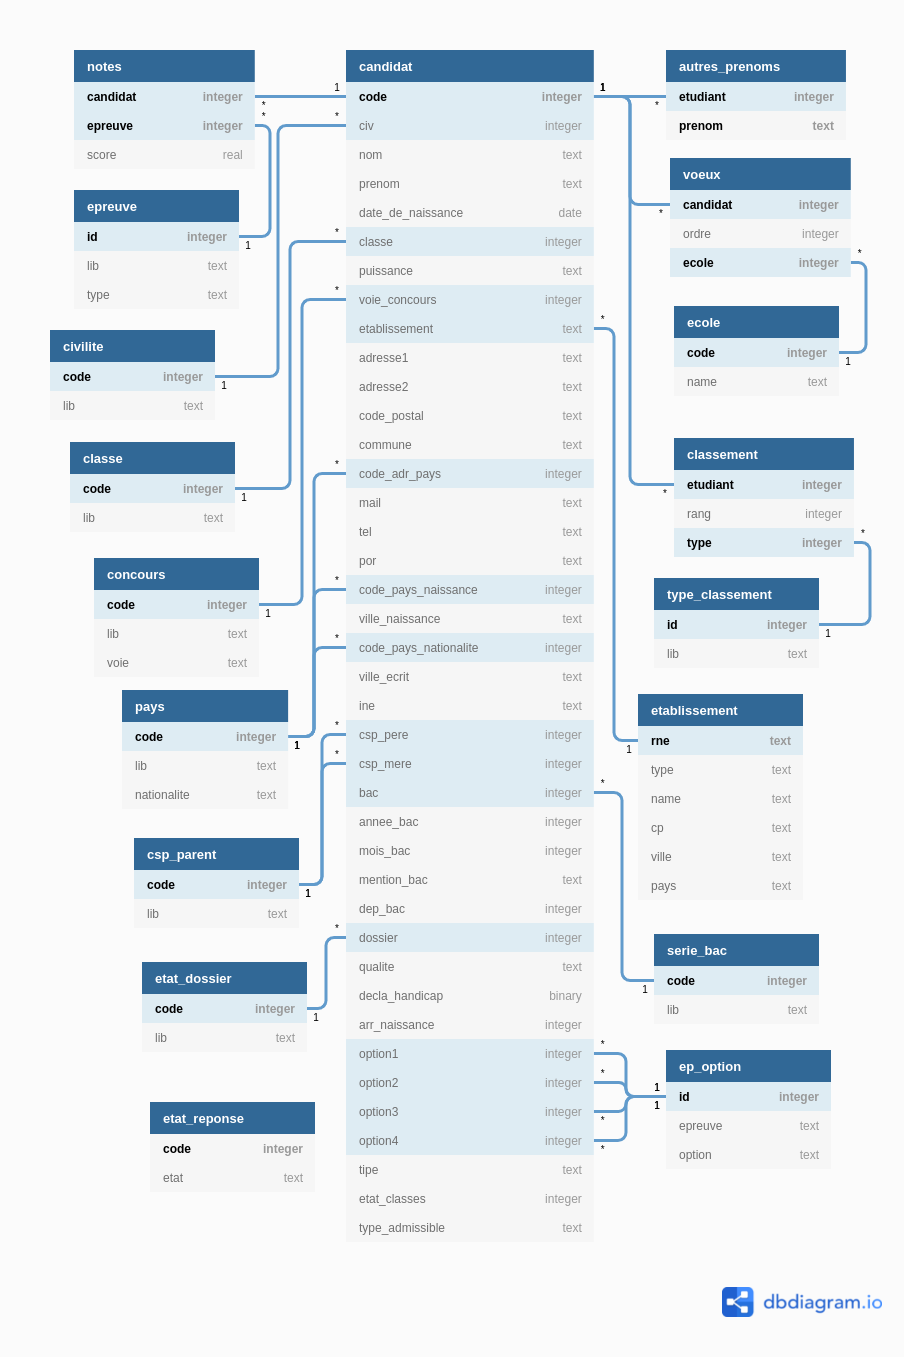
\includegraphics[scale = 0.49]{Images/Etat de l'art/schema_db.png}
                \caption{Schéma du modèle de données}
                \label{fig:bd}
            \end{figure}
            
            % \begin{figure}[!h]
            %     \centering
            %     \includegraphics[scale = 0.41]{Images/Etat de l'art/schéma_structure_2.png}
            %     \caption{Schéma du modèle de données 2e partie}
            %     \label{fig:bd2}
            % \end{figure}
            
        \newpage
        Chaque attribut de nos tables possèdent une valeur sémantiquement atomique, qui ne peut pas être divisé. Les attributs ne possèdent pas de valeurs multiples (listes, tableaux, etc.) ni de valeurs \texttt{NULL}, elles sont soit des \texttt{integer}, soit des \texttt{text}, et rarement des \texttt{binary} qui peuvent être ramenés à des \texttt{integer} (dans l'implémentation en \textsf{SQLite}, le \texttt{binary} n'existe pas, on utilisera un \texttt{integer}. De plus, les attributs non-clé dépendent de ou des attributs clés. Donc, le modèle est 1FN.
        
        En séparant les attributs clés et les attributs non-clé, dans chaque table les attributs non-clé dépendent de l'ensemble des attributs clés de la table. Les attributs en bleus sont des clés. Dans la table \texttt{classement}, le couple (\texttt{etudiant}, \texttt{type}) est une clé primaire, et \texttt{rang} désignant le rang dépend du candidat et du type de classement (admissible, admis, etc.)~; dans la table \texttt{voeux}, le couple (\texttt{candidat}, \texttt{ecole}) est une clé et \texttt{ordre} dépend de ce couple, car l'ordre des voeux est associé au candidat et à l'école concernée~; de même pour le couple (\texttt{candidat}, \texttt{epreuve}) dans la table \texttt{notes}, \texttt{score} (la note) n'a de signification que lorsqu'on précise le candidat et l'épreuve en question. Pour les autres tables, il n'y a qu'une seule clé, les attributs non-clé dépendent que de cette clé. Ainsi, dans toutes les tables, les attributs non-clé dépendent de la clé entière, le modèle est 2FN.
        
        Dans la table \texttt{candidat}, les attributs non-clé sont mutuellement indépendants, en particulier, pour les attributs \texttt{code\_postal} et \texttt{commune}, deux communes différentes peuvent avoir le même code postal, notamment les communes voisines. Par exemple, Carcès, Correns, Cotignac, Entrecasteaux et Montfort-sur-Argens ont le même code postal qui est 83570~\cite{cp}. De même pour la table \texttt{etablissement}, les attributs non-clé sont mutuellement indépendants. Les banques de concours ont pour la plupart des filières en commun, donc les attributs \texttt{concours.lib} et \texttt{concours.voie} sont indépendants. Tout comme le nom de l'épreuve et le type de l'épreuve, il peut y avoir une épreuve de mathématiques à l'écrit et à l'oral, donc les attributs \texttt{epreuve.lib} et \texttt{epreuve.type} sont indépendants. De même pour, les options des épreuves, le même type d'épreuve peut proposer des options différentes, par exemple, l'épreuve de Info./SI propose deux options, Sciences Industrielles et Informatique, donc les attributs \texttt{ep\_option.epreuve} et \texttt{ep\_option.option} n'ont pas de relation. Les autres tables n'ont qu'un seul attribut non-clé, dont nécessairement, ils dépendent de la clé de la table. De ce fait, le modèle de données est bien 3FN. 
        
    \subsection{Contraintes d'intégrité}
    
        Il a fallu contraindre notre base de données pour qu'elle ne prenne que des valeurs autorisées. Ces contraintes sont nécessaires pour que la base ne contiennent pas des données incohérentes ou incomplètes. Dans ce but, des contraintes ont été ajouté à certains champs des tables de la base de données. Listes du contenu des champs de la Figure~\ref{fig:bd}~:
        \begin{itemize}[label=\textbullet]
            \item \texttt{etat\_reponse.code}~: un entier, clé primaire~;
            \item \texttt{etat\_reponse.etat}~: du texte non vide~;
            \item \texttt{ecole.code}~: un entier, clé primaire~;
            \item \texttt{ecole.name}~: du texte, non vide~;
            \item \texttt{etablissement.rne}~: la rne de l'établissement et sert de clé primaire~;
            \item \texttt{etablissement.type}~: du texte~;
            \item \texttt{etablissement.name}~: du texte, non vide~;
            \item \texttt{etablissement.cp}~: du texte (certains codes postaux étrangers contiennent des lettres)~;
            \item \texttt{etablissement.ville}~: du texte, non vide~;
            \item \texttt{etablissement.pays}~: du texte~;
            \item \texttt{concours.code}~: un entier, clé primaire~;
            \item \texttt{concours.lib}~: du texte, non vide~;
            \item \texttt{concours.voie}~: du texte, non vide, couple unique avec \texttt{concours.lib}~;
            \item \texttt{voeux.candidat}~: un entier, non vide, clé étrangère provenant de \texttt{candidat.code}~;
            \item \texttt{voeux.ordre}~: un entier strictement supérieur à 0 et, non vide, forme un couple unique avec \texttt{voeux.candidat}~;
            \item \texttt{voeux.ecole}~: un entier, non vide, clé étrangère provenant de \texttt{ecole.code}, forme une clé primaire avec \texttt{voeux.candidat}~;
            \item \texttt{classement.etudiant}~: un entier, non vide, clé étrangère provenant de \texttt{candidat.code}~;
            \item \texttt{classement.rang}~: un entier strictement supérieur à 0 et non vide~;
            \item \texttt{classement.type}~: un entier, non vide, clé étrangère provenant de \texttt{type\_classement.id}, forme une clé primaire avec \texttt{classement.etudiant}~;
            \item \texttt{type\_classement.id}~: un entier, clé primaire~;
            \item \texttt{type\_classement.lib}~: du texte unique, non vide, on ne veut pas plus de une fois le même type de classement~;
            \item \texttt{epreuve.id}~: un entier, clé primaire~;
            \item \texttt{epreuve.lib}~: du texte, non vide~;
            \item \texttt{epreuve.type}~: du texte qui se trouve dans ECRIT, ORAL, SPECIFIQUE, CLASSEMENT~;
            \item \texttt{notes.candidat}~: un entier, non vide, clé étrangère provenant de \texttt{candidat.code}~;
            \item \texttt{notes.epreuve}~: un entier, non vide, clé étrangère provenant de \texttt{epreuve.id}, forme une clé primaire avec \texttt{notes.epreuve}~;
            \item \texttt{notes.score}~: un réel, non vide~;
            \item \texttt{autres\_prenoms.etudiant}~: un entier, non vide, clé étrangère provenant de \texttt{candidat.code}~;
            \item \texttt{autres\_prenoms.prenom}~: du text, non vide, forme une clé primaire avec \texttt{autres\_prenoms.etudiant}\footnote{on suppose que tout le monde n'a qu'un deuxième prénom, dans les données les candidats ont au plus un deuxième prénom}~;
            \item \texttt{pays.code}~: un entier, clé primaire~;
            \item \texttt{pays.lib}~: du text unique~;
            \item \texttt{pays.nationalité}~: du text unique~;
            \item \texttt{csp\_parent.code}~: un entier, clé primaire~;
            \item \texttt{csp\_parent.lib}~: du texte unique, non vide~;
            \item \texttt{serie\_bac.code}~: un entier, clé primaire~;
            \item \texttt{serie\_bac.lib}~: du texte unique, non vide~;
            \item \texttt{etat\_dossier.code}~: un entier, clé primaire~;
            \item \texttt{etat\_dossier.lib}~: du texte unique, non vide~;
            \item \texttt{ep\_option.id}~: un entier, clé primaire~;
            \item \texttt{ep\_option.epreuve}~: du texte, non vide~;
            \item \texttt{ep\_option.option}~: du texte, non vide, forme un couple unique avec \texttt{ep\_option.epreuve}~;
            \item \texttt{civilite.code}~: un entier, clé primaire~;
            \item \texttt{civilite.lib}~: du texte unique, non vide, en particulier M. et Mme~;
            \item \texttt{classe.code}~: un entier, clé primaire~;
            \item \texttt{classe.lib}~: du texte unique, non vide~;
            \item \texttt{candidat.code}~: un entier, clé primaire, représente le numéro scei du candidat~;
            \item \texttt{candidat.civ}~: une entier, non vide, clé étrangère provenant de \texttt{civilite.code}~;
            \item \texttt{candidat.nom}~: du texte, non vide~;
            \item \texttt{candidat.prenom}~: du texte, non vide~;
            \item \texttt{candidat.date\_de\_naissance}~: du type date~;
            \item \texttt{candidat.classe}~: un entier, clé étrangère provenant de \texttt{classe.code}~;
            \item \texttt{candidat.puissance}~: du texte à prendre dans 3/2, 5/2, 7/2~;
            \item \texttt{candidat.voie\_concours}~: un entier, clé étrangère provenant de \texttt{concours.code}~;
            \item \texttt{candidat.etablissement}~: du texte, clé étrangère provenant de \texttt{etablissement.rne}~;
            \item \texttt{candidat.adresse1}~: du texte, non vide~;
            \item \texttt{candidat.adresse2}~: du texte~;
            \item \texttt{candidat.code\_postal}~: du texte (car pourrait contenir des lettres, non vide~;
            \item \texttt{candidat.commune}~: du texte, non vide~;
            \item \texttt{candidat.code\_adr\_pays}~: un entier, non vide, clé étrangère provenant de \texttt{pays.code}~;
            \item \texttt{candidat.mail}~: du texte, non vide~;
            \item \texttt{candidat.tel}~: du texte (car il peut y avoir +33(0)1)~;
            \item \texttt{candidat.por}~: du texte (car il peut y avoir +33(0)6)~;
            \item \texttt{candidat.code\_pays\_naissance}~: un entier, non vide, clé étrangère provenant de \texttt{pays.code}~;
            \item \texttt{candidat.ville\_naissance}~: du texte~;
            \item \texttt{candidat.code\_pays\_nationalite}~: un entier, non vide, clé étrangère provenant de \texttt{pays.code}~;
            \item \texttt{candidat.ville\_ecrit}~: du texte~;
            \item \texttt{candidat.ine}~: du texte unique~;
            \item \texttt{candidat.csp\_pere}~: un entier, clé étrangère provenant de \texttt{csp\_parent.code}~;
            \item \texttt{candidat.csp\_mere}~: un entier, clé étrangère provenant de \texttt{csp\_parent.code}~;
            \item \texttt{candidat.bac}~: un entier, clé étrangère provenant de \texttt{serie\_bac.code}~;
            \item \texttt{candidat.annee\_bac}~: un entier~;
            \item \texttt{candidat.mois\_bac}~: un entier~;
            \item \texttt{candidat.mention\_bac}~: du texte, TB, B, AB, S~;
            \item \texttt{candidat.dep\_bac}~: un entier, département d'obtention du BAC~;
            \item \texttt{candidat.dossier}~: un entier, clé étrangère provenant de \texttt{etat\_dossier.code}~;
            \item \texttt{candidat.qualite}~: du texte~;
            \item \texttt{candidat.decla\_handicap}~: un entier, 0 ou 1, par défaut 0~;
            \item \texttt{candidat.arr\_naissance}~: un entier, par défaut 0~;
            \item \texttt{candidat.option1}~: un entier, clé étrangère provenant de \texttt{ep\_option.id}~;
            \item \texttt{candidat.option2}~: un entier, clé étrangère provenant de \texttt{ep\_option.id}~;
            \item \texttt{candidat.option3}~: un entier, clé étrangère provenant de \texttt{ep\_option.id}~;
            \item \texttt{candidat.option4}~: un entier, clé étrangère provenant de \texttt{ep\_option.id}~;
            \item \texttt{candidat.tipe}~: du texte~;
            \item \texttt{candidat.etat\_classes}~: un entier~;
            \item \texttt{candidat.type\_admissible}~: du texte\footnote{lettre entre A et B}.
        \end{itemize}

\newpage

%%%%% Algorithmes %%%%%
\section{Implémentation et application des algorithmes}
% titre à modifier peut-être

Tout d'abord, nous avons écrit des algorithmes permettant de remplir la base de données à partir des fichiers excel fournis~\cite{excel}, puis ces codes ont été regroupés dans un seul script et optimisé. Ensuite, un script de test de cohérence a été fait pour vérifier la cohérence des fichiers. Et enfin, nous avons réalisé l'application de gestion avec les fonctionnalités décrites qui font appel à du SQL pour récupérer les informations dans la base de données.

    \subsection{Script de remplissage de la base de données}
        % Parler du remplissage de la bd avec les scripts + regroupement des scripts et optimisation
        %technos utilisées, script création des tables
        Pour gérer notre base de donnée, nous utilisons le système de gestion de base de données \textsf{SQLite 3} et le langage \textsf{SQL}.
        L'initialisation de la base de données est faite grâce au fichier \texttt{createdb.sql} qui crée toutes les tables de notre modèle et rempli les tables civilite et type\_classement.
        Ce fichier peut être exécuté avec \textsf{SQLite} mais notre script qui importe le reste des données permet aussi de l'exécuter.
        Les scripts de cette partie ont été écrits dans le langage \textsf{Python 3} avec les modules suivant :
        \begin{itemize}[label=-]
            \item \textsf{pandas} : permet de lire les fichier \texttt{.csv} et \texttt{.xlsx} et permet de nommer les colonnes des tableurs~\cite{pd};
            \item \textsf{openpyxl} : lit uniquement les fichiers \texttt{.xlsx} et ne permet pas de nommer les colonnes mais charge les tableurs plus rapidement~\cite{xl};
            \item \textsf{sqlite3} : permet la connexion avec la base de donnée~\cite{sqlite};
            \item \textsf{click} : permet l'intégration du script dans une interface en ligne de commande;
            \item \textsf{pathlib} : permet de gérer facilement les chemins systèmes.
        \end{itemize}
        
        % Idée de sous-parties
        \subsubsection{Algorithmes de remplissage}
            % Explication du code
            Nous chargeons les tableurs l'un après l'autre et remplissons les tables en fonction des données contenues dans ces fichiers. Tous les fichiers sont traités de façon similaire mais le code a du être adapté aux caractéristiques de chaque fichier.
            
            La fonction suivante est un exemple type de la façon dont nous avons rempli la base de donnée. Elle remplit la table ecole depuis les données du fichier \texttt{listeEcoles.xlsx}.
            Le paramètre \verb|database| est la connexion vers la base de donnée et \verb|path| est le chemin du dossier contenant les tableurs. La méthode \verb|c.execute| permet de d'exécuter une commande \textsf{SQL}. Ici elle insère un couple de donnée dans la table ecole.

            \begin{verbatim}
    def import_ecole(database: sql.Connection, path: Path):
        data = pd.read_excel(path/'listeEcoles.xlsx', header=0)
        c = database.cursor()
        for i in range(len(data)):
            nom = data['Nom _ecole'][i]
            code = int(data['Ecole'][i])
            c.execute("INSERT INTO ecole VALUES (?,?)", (code, nom))
            \end{verbatim}
            
        \subsubsection{Regroupement des scripts et optimisation}
            % Explication des choix
            Nous nous sommes réparti l'écriture des fonctions donc nous avons dû regrouper les différents morceaux de code. Cette phase c'est accompagné d'une optimisation du code.
            Ainsi nous ne chargeons qu'un fichier à la fois et chaque fichier n'est chargé qu'un seule fois. De cette façon le temps de chargement des fichiers et la charge mémoire sont réduits au maximum.
            
            L'ordre de traitement des données est défini de façon à s'aider de tables précédemment remplies.
            Par exemple pour les candidats provenant de la filière ATS nous n'avons que le nom du pays de leur adresse. Or la clé étrangère à mettre dans la table candidat est le code du pays. Nous devons donc rechercher dans la table pays le code correspondant. Si il n'existe pas déjà nous l'ajoutons à la table.
            
            Enfin une première review du code a été faite pour éliminer les parties dupliquées ou trop ressemblantes. Elles ont été remplacées par des appels à des fonctions.
        
        \subsubsection{Algorithme du script de test de cohérence}
        
        Comme pour tester la cohérence des données nous n'effectuons que des requêtes \textsf{SQL}, tous les identifiants des données à tester ont été mis dans un fichier texte. Il est construit selon l'exemple suivant~:
        
        \begin{verbatim}
ADMIS_ATS.xlsx;ADMIS_MP-SPE.xlsx
    	Can _cod;pk
    	Civ _lib;civilite;ci;ci.lib;J;candidat;ca;ca.civ=ci.code;W;ca.code
        \end{verbatim}
        
        Une première ligne sans tabulation est la liste des fichiers pour lesquels les lignes suivantes vont se référer.
        Les lignes suivantes commencent avec une tabulation et le premier champs correspond a un nom de colonne des tableurs. Les champs suivants caractérisent cette colonne.
        Si il y a \verb|pk|, alors cette colonne va servir de clé primaire pour identifier l'enregistrement à vérifier. 
        Sinon l'ensemble des champs suivants décrivent la requête \textsf{SQL} a effectué.
        Les 3 premiers champs indiquent la table et le nom du champs de la table à récupérer.
        Le champs \verb|J| (qui est optionnel) et les 3 suivants indique une jointure a effectué et le champs \verb|W| et le suivant caractérise la partie \verb|WHERE| de la requête.
        
        Pour résumer, chaque ligne suit la grammaire suivante : 
        
        \begin{center}
        $\{(L,F,P,A,S,J),(\texttt{;},\texttt{pk},\texttt{J},\texttt{W},\texttt{\textbackslash t},statements),\rightarrow,L\}$
        \begin{equation*}
            \begin{cases}L\rightarrow F|P
            \\F\rightarrow filename|filename\texttt{;}F
            \\P\rightarrow column\_header\texttt{;}A
            \\A\rightarrow \texttt{pk}|S\end{cases}
            \begin{cases}S\rightarrow table\texttt{;}table\_alias\texttt{;}column\_name\texttt{;}JW
            \\J\rightarrow \epsilon|\texttt{J}\texttt{;}table\texttt{;}table\_alias\texttt{;}on\_statement\texttt{;}
            \\W\rightarrow \texttt{W}\texttt{;}where\_statement\end{cases}
        \end{equation*}
        %\caption{Caption}
        %\label{fig:my_label}
        \end{center}
        
        \subsubsection{Interface en ligne de commande}
        Grâce au module Click, l'ensemble des scripts pour la création, le remplissage et la vérification (voir section~\ref{parag:coherence}) ont été regroupés dans une unique commande.
        La commande prend en paramètre les chemins vers les différents fichiers nécessaire et comme option les différentes étapes à exécuter.
        \\
        Exemple d'utilisation :
        \begin{verbatim}
        importxl concours.db files/ --init createdb.sql --import --verif
        \end{verbatim}
        Ici les fichiers tableurs sont situés dans le dossier \verb|files/| et la base de donnée \verb|concours.db| est initialisée avec le fichier \verb|createdb.sql|. La commande effectue aussi l'importation et la vérification des données.
        
    
    \newpage
    \subsection{Application web}
        \subsubsection{Outils utilisés}

            Pour la conception de notre application web, nous avons décidé de rester sur Python car c'est un langage intuitif, très flexible et qui possède plusieurs librairies qui facilitent le développement web et la manipulation de bases de données (et c'est aussi le langage que nous avons utilisé en WebBd).
            
            La partie Back-end de notre application repose essentiellement sur \textsf{Flask} et \textsf{SQLite3} qui sont deux framework disponibles sur \textsf{Python}.
            \begin{itemize}

            \item \textsf{Flask} est un un micro-framework simple et léger qui permet, entre autres,  de créer un serveur de développement et de débugage ainsi qu'un moteur de template pour le rendu \textsf{HTML}.
            \item \textsf{SQLite3} est une bibliothèque qui propose un moteur de base de données relationnelle accessible par le langage \textsf{SQL} et qui nous permet donc d'interroger facilement notre base de données.
             \end{itemize}
             
             Pour la partie Front-end nous avons utilisé \textsf{HTML} et \textsf{CSS} ainsi que le framework \textsf{Bootstrap} pour la création du design (barre de navigation, formulaires, tableaux...).
             

             

            \subsubsection{Fonctionnalités}
            Le fichier \texttt{app.py} contient toutes les fonctions créées avec \textsf{Flask} et \textsf{SQLite3}. Pour lancer l'application, il suffit d'entrer l'adresse \texttt{http://127.0.0.1:5000/X}  dans votre navigateur web - après l'installation et la configuration de \textsf{Flask} bien entendu \textit{(voir le fichier README.md du dépôt Git)} où X est l'une des 'routes' suivantes : 
            \begin{itemize}[label=\textbullet]
            \item \texttt{ecole} : Affiche l'ensemble des écoles du Concours Mines-Télécom, voir l'exemple ci-dessous.
            \item \texttt{etablissement} : Affiche les établissements des candidat, avec le RNE, le type, le nom, le code postal, la ville et le pays de chaque établissement.
            \item \texttt{epreuve} : Affiche la liste de toutes les épreuves du concours avec leurs numéros et leurs types.
            \item \texttt{option} : Affiche la liste des épreuves en option.
            \item \texttt{csp} : Affiche l'ensemble des catégories socioprofessionnelles des parents des candidats.
            \item \texttt{candidatByCode/code} : Affiche l'ensemble des informations du candidat numéro \texttt{code}, telles que son code, son nom et prénom, son adresse, sa classe, son établissement, etc.
            \item \texttt{voeux/code} : Affiche la liste des vœux présentés par le candidat numéro \texttt{code}.
            \item \texttt{notes/code} : Renvoie la liste des notes obtenues par le candidat numéro \texttt{code}.
            \item \texttt{classement/code} : Donne les différents rangs du candidat numéro \texttt{code} avec le type correspondant (rang de l'épreuve écrite, de l'épreuve orale, d'admissibilité ou le rang de classe).
            \item \texttt{rech} : Permet de trouver un candidat à partir de son nom. A savoir qu'il n'est pas nécessaire de fournir le nom complet du candidat : Par exemple si on tape \texttt{ben} nous obtenons la liste de tous les candidats pour lesquels le nom contient la chaîne de caractères \texttt{ben}, voir l'exemple ci-dessous.
            \item \texttt{moyenne/codepreuve/rne} : Permet d'obtenir la moyenne sur l'épreuve numéro \texttt{codepreuve} pour les candidats venant de l'établissement numéro \texttt{rne}.
            \end{itemize}
            
                \begin{figure}[!h]
        \centering
        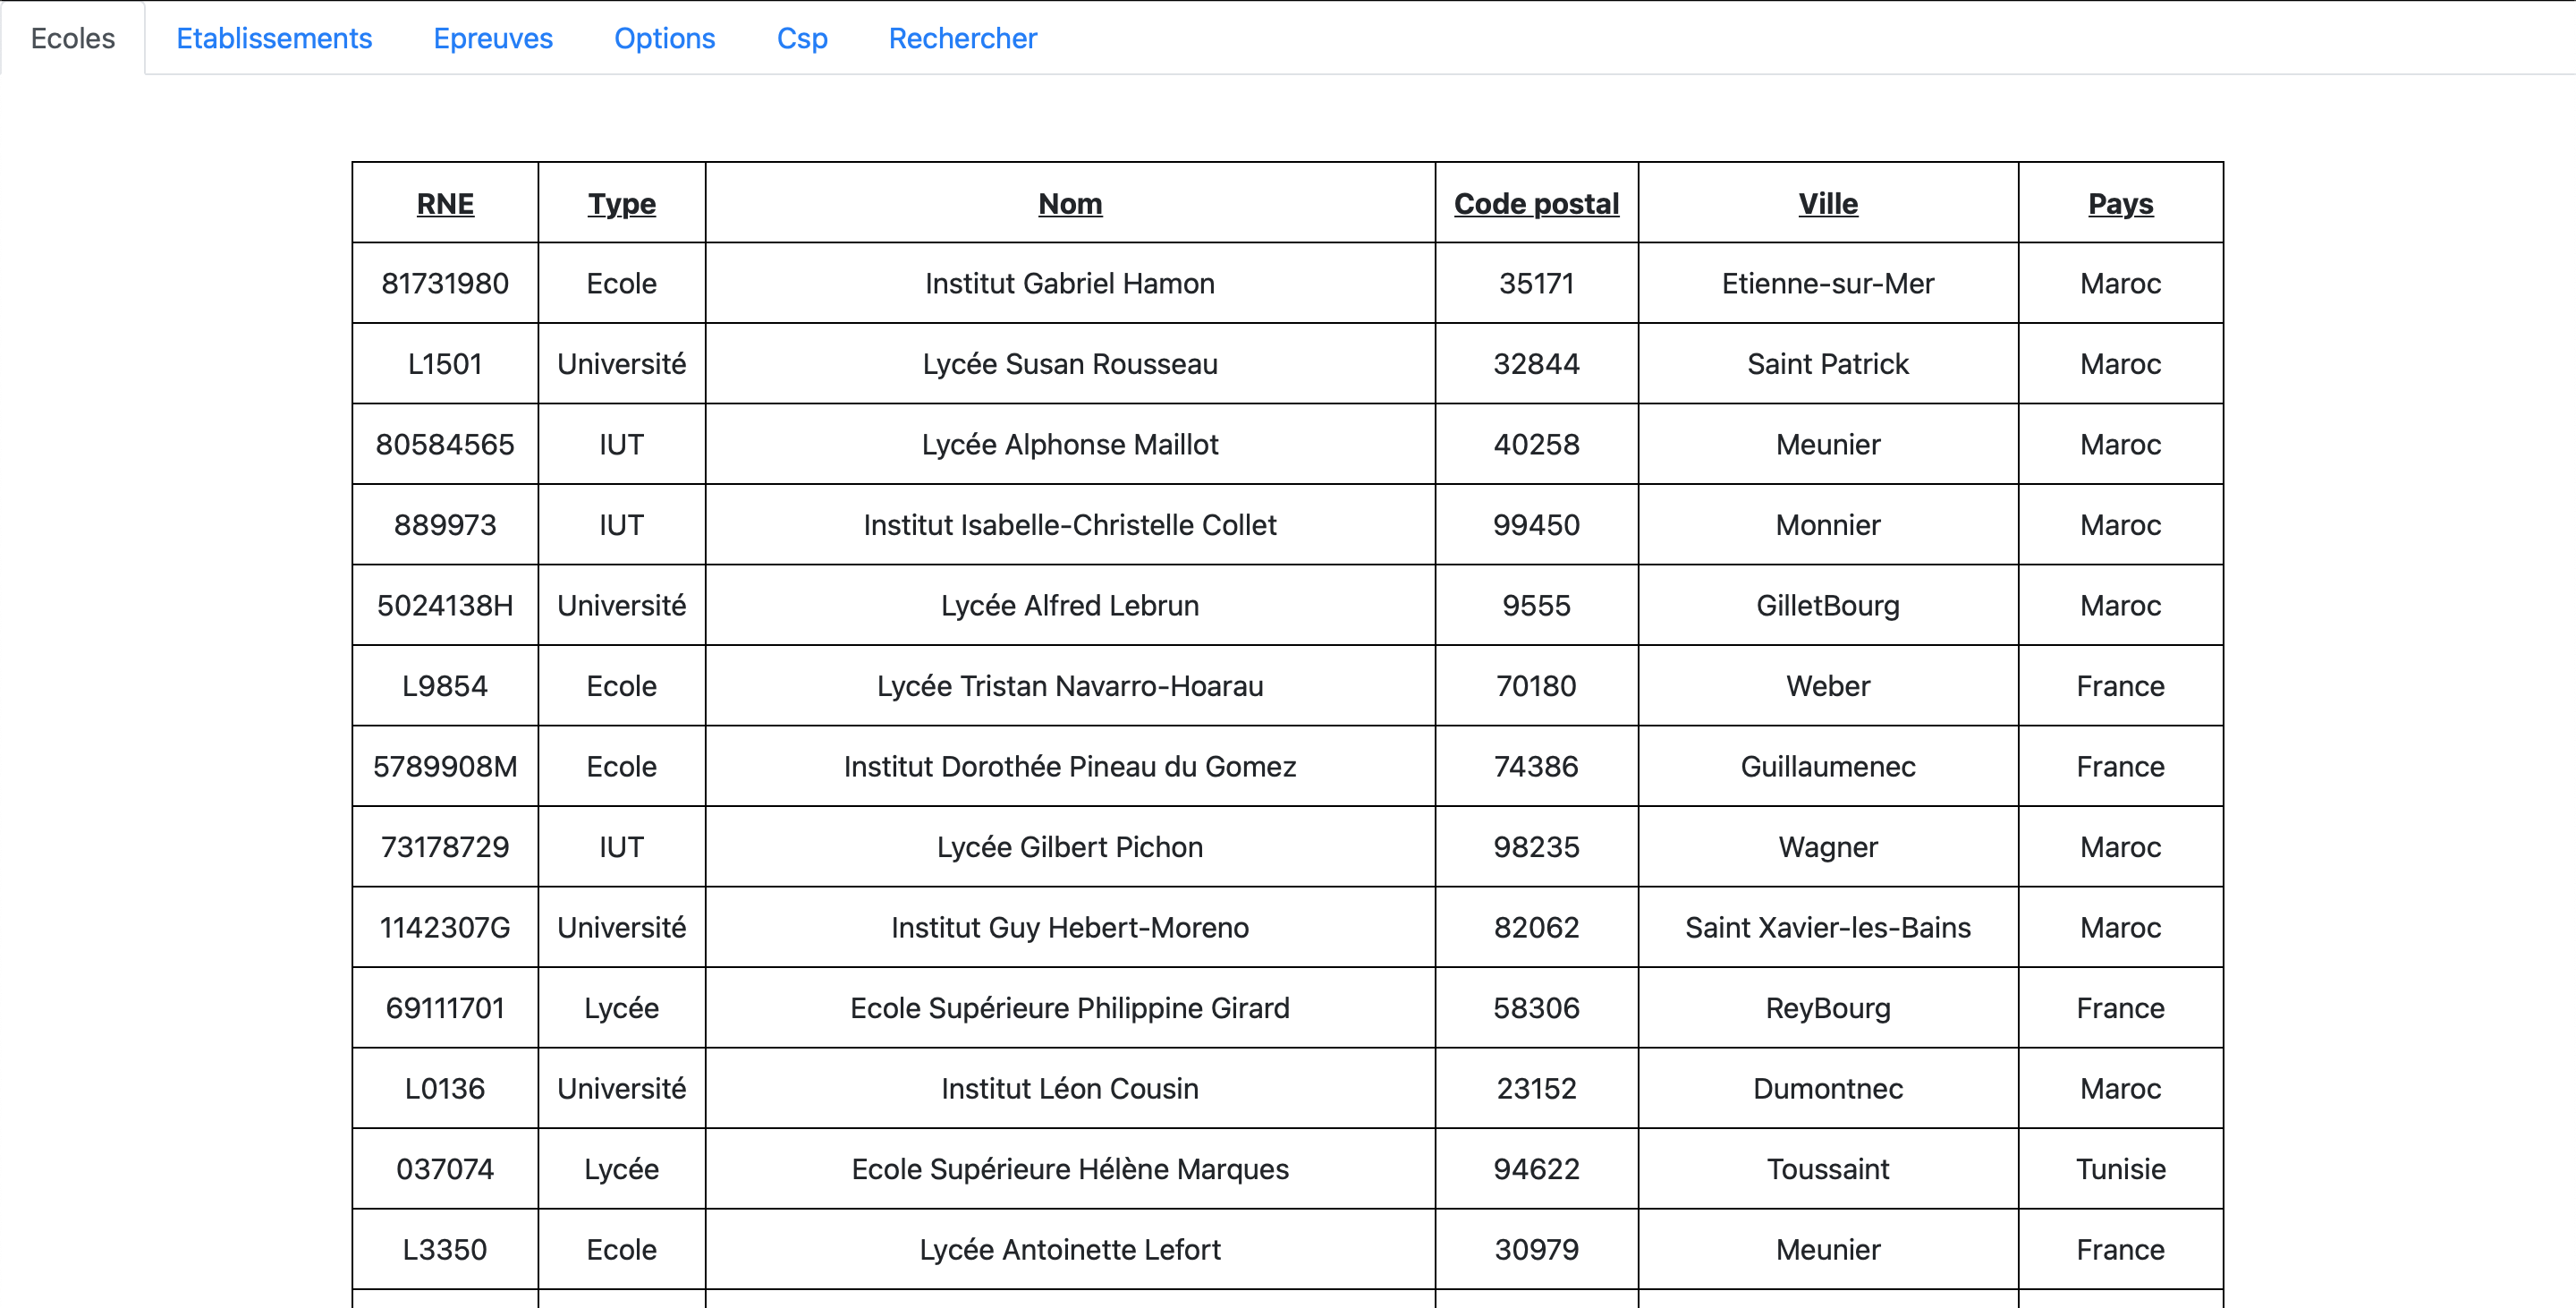
\includegraphics[scale = 0.4]{Images/App/ecoles.png}
        \caption{Résultat de \textit{http://127.0.0.1:5000/rech}}
    \end{figure}
    
                   \begin{figure}[!h]
        \centering
        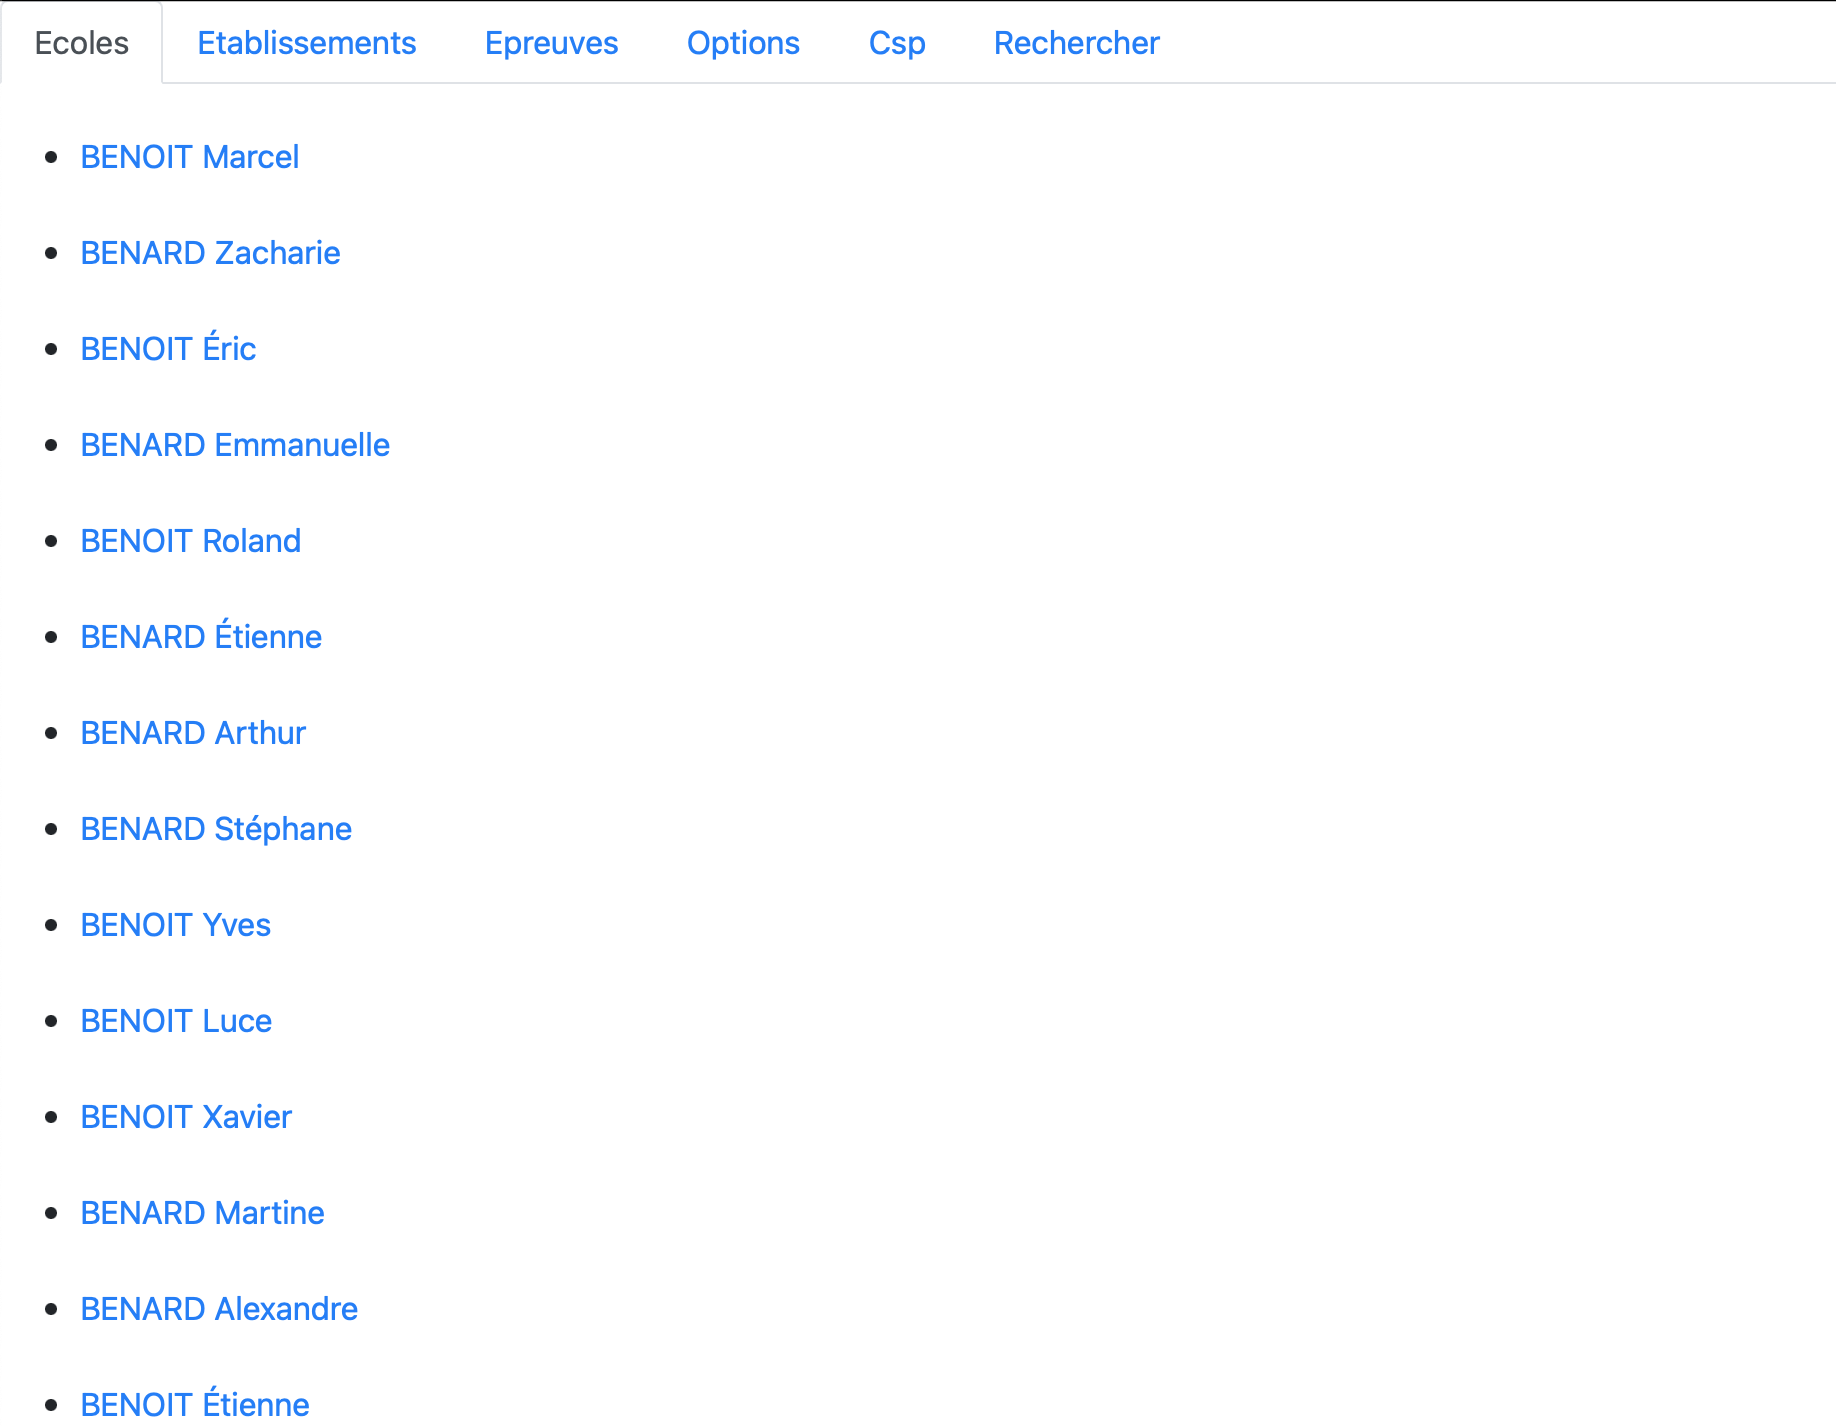
\includegraphics[scale = 0.4]{Images/App/rech.png}
        \caption{Résultat de la recherche des noms contenant 'ben'}
    \end{figure}

        
   

       
            

\newpage

%%%%% Test et cohérence %%%%%
\section{Tests de cohérence et de performance}
    \subsection{Cohérence} \label{parag:coherence}
        % Expliquer la notion de cohérence et le procédé de vérification
        Après l'importation des données dans la base, nous avons effectué une vérification de la cohérence de celles-ci. Cette vérification est constituée de trois étapes.

        Premièrement les contraintes d'intégrité lèvent des erreurs si les données mises dans les tables ne respectent pas certaines caractéristiques.

        Deuxièmement nous vérifions l'existence de toutes les clé étrangères. Pour cela nous utilisons la commande \verb|PRAGMA foreign_key_check| présente dans \textsf{SQLite} qui renvoie la liste de toutes les clés étrangères problématiques. Lors de l'exécution de cette commande, nous nous somme aperçu que certains candidats venaient d'établissements non présents dans la table du même nom et que certaines notes et rangs référaient à des candidats inconnus. Nous avons décidé de complété la table établissement pour le premier cas et de supprimer les enregistrements problématiques pour le second. Si d'autres enregistrements réfèrent à des candidats inconnus, ils seront supprimés sinon ils seront affiché sur la sortie standard.
        
        Troisièmement nous vérifions la cohérence des informations entre celles de la base de donnée et celles des fichiers non utilisé pour la remplir. Car, comme certaines données sont redondantes à travers plusieurs fichiers, nous ne les récupérons que dans un seul. Il faut alors vérifier si certaines informations ne sont pas contradictoires entre ces fichiers. Le script qui s'occupe de ça ne fait qu'afficher les éventuelles erreurs. 
        
        Le script a relevé une erreur, un candidat se trouvait être 3/2 est peut-être 5/2.
        
    \subsection{Performance}
        % Présenter l'exigence du temps d'exécution et explique les solutions d'optimisation
        Le script qui initialise et rempli la base de donnée met environ 40 secondes à s'exécuter. Cependant, le script qui vérifie la cohérence des données met environ 2 minutes.

\newpage

%%%%% Gestion de Projet %%%%%
\section{Gestion de projet}
    Cette partie est consacrée à la présentation de notre gestion de projet. L'équipe s'est inspirée du cadre méthodologique SCRUM, pour l'organisation du groupe et du projet, voir la table~\ref{tab:roles}, la méthode SMART a été utilisé pour le découpage des tâches, voir la table~\ref{tab:SMART}; avant le début du projet une analyse des risques en utilisant la matrice SWOT a été effectuée, voir la figure~\ref{tab:swot}.
    \subsection{Équipe de projet}
    Ce projet a été réalisé par le groupe 9 dont les membres sont~:
    \begin{itemize}[label=\textbullet]
        \item Maël SAILLOT, le développeur responsable du dépôt \textsf{git}, il s'assure de l'organisation du dépôt, il vérifie les lignes de codes (\textsl{code review}) et les optimise, il s'occupe de régler les soucis informatique au sein du projet;
        \item Céline ZHANG, le développeur chef de projet, elle s'occupe de l'organisation des réunions, du déroulement des réunions, du découpage et de la répartition des tâches, de l'avancée du rapport, et elle se charge de rédiger les comptes rendus de réunions;
        \item Ahmed ZIANI, le développeur responsable du contrôle, il s'occupe l'exactitude des notions abordées, vérifie les sources de celles-ci, la bonne application des règles de constructions de la base de données.
    \end{itemize}
Chaque membre est développeur, donc participe à la conception et à l'écriture des codes.%, en plus des rôles complémentaires spécifiques.
    \begin{table}[!h]
    \begin{center}
        \begin{tabular}{|l|l|}
        \hline
            Membre de l'équipe 9 & Rôles ou charges \\
        \hline
        \hline
            Céline ZHANG & leader \\
        \hline
            Ahmed ZIANI & reviewer \\
        \hline
            Maël SAILLOT & responsable du git \\
        \hline
        \end{tabular}\\
    \end{center}
    \caption{Tableau des rôles}
    \label{tab:roles}
    \end{table}


\subsection{Analyse du projet}

\subsubsection{Définition des objectifs}
Les objectifs ont été définis en se basant sur la méthode SMART comme indiqué sur la table~\ref{tab:SMART}: 
\begin{table} [!h]
 \begin{center}
 \begin{tabular}{|c||l|l|}
 \hline
  & Critère & Indicateur \\
 \hline
 S & Spécifique & Objectif clair, précis et sans ambiguité \\
 \hline
 M & Mesurable & Objectif quantifié permettant de mesurer l'état d'avancement \\
 \hline
 A & Ambitieux et Atteignable & Objectif représentant un défi atteignable et non démotivant \\
 \hline
 R & Réaliste & Objectif envisageable et suffisamment motivant \\
 \hline
 T & Temporellement défini & Objectif défini et délimité dans le temps \\
 \hline
 \end{tabular}
 \end{center}
 \caption{La méthode SMART}
 \label{tab:SMART}
 \end{table}

%%\begin{spacing}
\newpage
\subsubsection{Analyse des risques: Matrice SWOT}
    Nous avons évalué les risques du projet en utilisant la matrice SWOT sur la figure.
    \begin{table}[!h]
        \centering
        \begin{tabular}{|c|c|}
            \hline
            \textbf{Forces} & \textbf{Faiblesses} \\
            \hline
            \hline
                    & \\
            Expérience en projet d'équipe & Première coopération avec les membres \\ 
                    & \\
            Compétences en Python et en \LaTeX & Consignes ambiguës et incomplets \\
                    & \\
            Quelques connaissances en développement \textsl{Web} & Pas assez de connaissances avancées en \textsl{Web}  \\
                    & \\
            Connaissances en \textsf{SQL} & Première réalisation d'une base de données \\
                    & \\
            \hline
            \hline
            \textbf{Opportunités} & \textbf{Menaces} \\
            \hline
            \hline
             & \\
            Possibilité de demander de l'aide aux 2A et 3A & Temps réduit avec les partiels \\
             & \\
            Obtenir l'aide des professeurs & Situation sanitaire \\
             & \\
            \hline
        \end{tabular}
        \caption{Matrice SWOT du projet}
        \label{tab:swot}
    \end{table}

\newpage
\subsubsection{Répartition des tâches : Matrice RACI}

    %\addcontentsline{toc}{section}{Répartition des tâches : Matrice RACI}
     Nous avons transformé les objectifs en tâches énumérées dans notre matrice RACI. \\
    %\newline

\begin{table}[!h]
    \centering
    \begin{tabular}{|l|c|c|c|c|l|}
         \hline
         & \textbf{Ahmed} & \textbf{Céline} & \textbf{Maël}    \\
         \hline
         \hline
        Phase 1 : Conception de la base de données \\
         \hline
         \hline
         Schémas sur dbdiagram.io & CI & R & RA   \\
         \hline
         Contraintes d'intégrité & R & CI & RA  \\
         \hline
         Formes normales & R & R & R  \\
         \hline
         Fichier createdb.sql & R & RA & R  \\
         \hline
         \hline
         Phase 2 : Importation des données et tests \\
        \hline
        \hline
        Scripts d'importation de données & RA & R & R \\
        \hline
        Regroupements des codes & I & I & RA \\
        \hline
        Tests de cohérence & CI & CI & RA \\
        \hline
        \hline
        Phase 3 : Application Web \\
        \hline
        \hline
        Conception Back-end & RA & R & CI \\
        \hline

        Conception Front-end & R & RA & R \\

        \hline
        
    \end{tabular}
    \caption{Matrice RACI}
    \label{tab:raci}
\end{table}

 
    \subsubsection*{Légende}
    %%\begin{spacing}{0.9}
    \noindent R : réalisateur. \\
    A : avoir l'autorité. \\
    C : conseiller. \\
    I : informé. \\
%%\end{spacing}

%%\end{spacing}

%\newpage

\subsection{Organisation du projet}
\subsubsection{Durée}
Le projet a commencé 3 Avril 2021 et s'est terminé le 11 Juin 2021, pour une durée de 68 jours. Cette version du rapport a été terminée le 11 Juin 2021.

\subsubsection{Le cadre méthodologique SCRUM}
% SCRUM est un cadre méthodologique et non pas une méthode.

Pour une meilleure organisation, nous avons choisi d'adapter une gestion de projet agile avec SCRUM. On a estimé que l'adaptation collective et rapide sera plus productive et plus constructive pour tous les membres de l'équipe.

Par conséquent, nous nous sommes basés sur les 3 piliers fondamentaux de SCRUM: 
\begin{itemize}[label=\textbullet]
    \item Transparence (visibilité concrète sur la situation)
    \item Inspection (détection des écarts par rapport aux objectifs)
    \item Adaptation (réctification de ces écarts par rapport aux objectifs)
\end{itemize}

Conformément à ce cadre, un ordonnancement du product backlog a été effectué, au début. Nous avons divisé les tâches sur des \textsl{sprints} fixés afin de pouvoir concevoir, réaliser et tester les nouvelles fonctionnalités au fur et à mesure.
En effet, pour chaque \textsl{sprint} on fixe un objectif à court terme et on se lance dans la réalisation. Une fois cet objectif atteint, nous discutons et nous nous adaptons à la situation, à travers les réunions hebdomadaires. \\
Toutes ces organisations ont été mis en oeuvre dans le tableau Trello\footnote{\url{https://trello.com/b/A4OHOVP4/projetpii-grp09}} comme illustré dans la figure~\ref{fig:exTrello02062021}.
    \begin{figure}[!h]
        \centering
        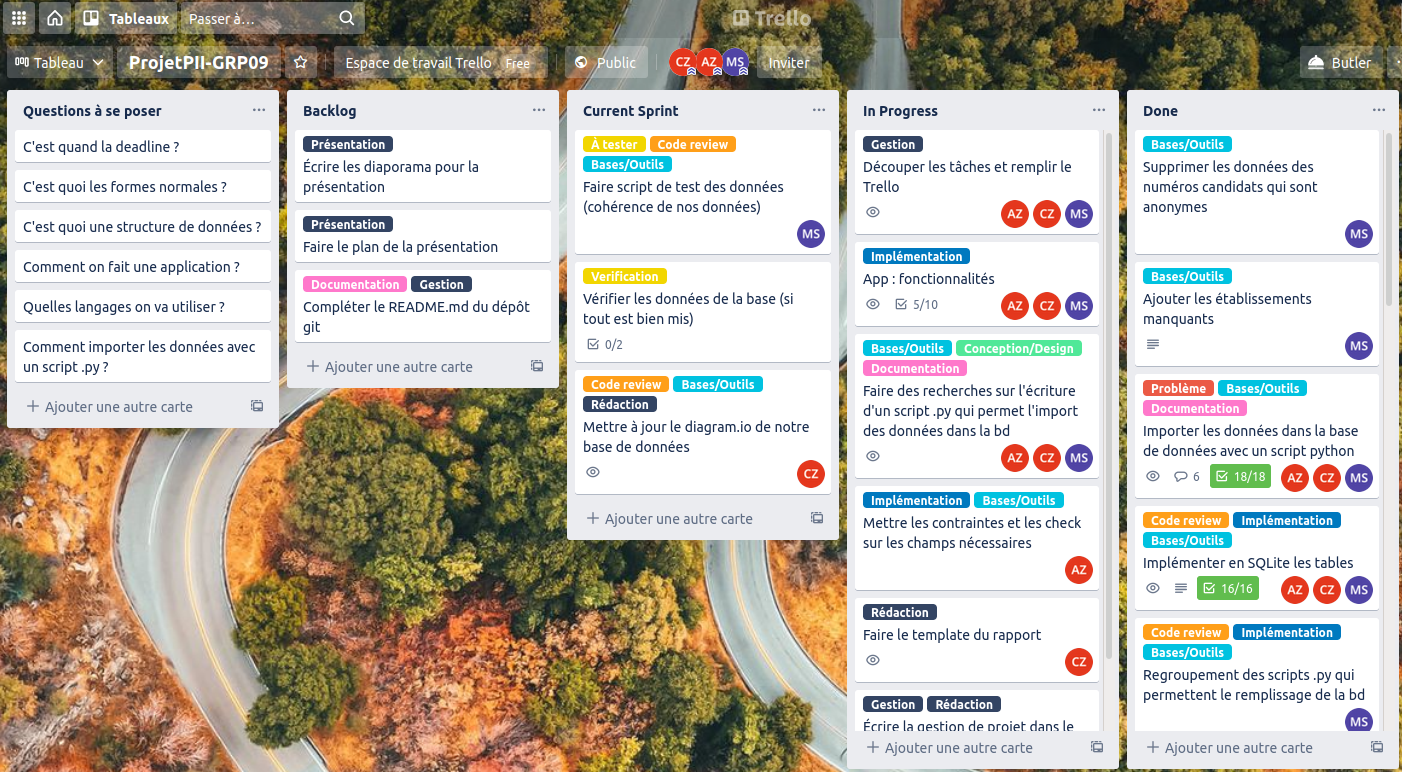
\includegraphics[scale = 0.365]{Images/Gestion de Projet/Trello/Trello_02062021.png}
        \caption{L'organisation du projet sur Trello}
        \label{fig:exTrello02062021}
    \end{figure}

\noindent L'organisation du tableau Trello était comme suit~:
\begin{itemize}[label=\textbullet]
    \item \textbf{Question à se poser :} les interrogations nécessaires~;
    \item \textbf{Backlog :} la liste de tâches priorisées~;
    \item \textbf{Current Sprint :} les tâches à réaliser au cours du \textsl{sprint} actuel~;
    \item \textbf{In Progress :} les tâches en cours de réalisation~;
    \item \textbf{Done :} les tâches finies.
\end{itemize}
Pour chaque tâche, il y a un ensemble d'étiquettes qui permettent de caractériser une tâche facilitant le traitement de celle-ci.
On distingue principalement des étiquettes qui précisent la nature ou l'avancement des tâches comme~:
\begin{itemize}[label=\textbullet]
    \item \textbf{Documentation :} la phase de documentation~;
    \item \textbf{Conception/Design :} la phase de la conception de l'algorithme.
    \item \textbf{Implémentation :} la phase de l'implémentation de l'algorithme~;
    \item \textbf{Code Review :} une étiquette qui est attribuée à la tâche après l'implémentation pour que les autres développeurs passent vérifier le code~;
    \item \textbf{À tester :} la phase des tests~;
    \item \textbf{Bases/Outils :} production d'élément nécessaire à l'implémentation de l'application~;
    \item \textbf{Vérification :} une tâche de vérification~;
    \item \textbf{Problème :} la tâche rencontre un problème~;
    \item \textbf{Gestion :} la tâche est en lien avec la gestion du projet~;
    \item \textbf{URGENT :} la tâche doit être traité très rapidement~;
    \item \textbf{Rédaction :} la tâche est en relation avec la rédaction du rapport~;
    \item \textbf{Présentation :} la tâche est en relation avec la réalisation de la présentation.
    % \item \textbf{Bug Proof :} quand une tâche est finie, on attribue cette étiquette et on la glisse dans la colonne Production.
    % \item \textbf{Flex :} des tâches supplémentaires non demandées par l'énoncé.
\end{itemize}

%%% Outils de travail %%%
\subsection{Outils de travail}

    \subsubsection{Communication}
    Les principaux outils de communication sont~: \textsf{Discord}, \textsf{Messenger}.
    \paragraph{\textsf{Discord}} a été utilisé pour communiquer en messages, pour organiser des réunions, montrer les codes, diffuser des explications, et éventuellement envoyer des documents.
    \paragraph{\textsf{Messenger}} est principalement utilisé pour la communication des réunions, l'échange des disponibilités et la discussion des particularités des tâches lors des \textsl{sprint} en dehors des réunions, pour régler un problème ou poser une question rapidement par exemple.
    
    \subsubsection{Programmation}
    Selon les préférences de chaque membre, plusieurs outils pour la programmation ont été utilisés.
    \begin{itemize}[label=\textbullet]
        \item Les langages et les modules: \textsf{Python}, \textsf{Pandas}, \textsf{Openpyxl}, \textsf{Flask}.
        \item Les IDE~: \textsf{PyCharm}, \textsf{Visual Studio Code}.
        \item Les consoles/logiciels~: \textsf{shell}, \textsf{PowerShell}, \textsf{SQLite3}, \textsf{SQLiteStudio}.
        \item Représentation de la base de données~: \textsf{dbdiagram.io}\footnote{\url{https://dbdiagram.io/home}}
    \end{itemize}
    
    \subsubsection{Partage du travail}
    Tout au long du projet, nous avons utilisé essentiellement le dépot \textsf{GitLab} fournit par l'école. Nous avons travaillé sur plusieurs branches. Notre dépôt a plusieurs répertoires pour organiser nos fichiers~:
    \begin{itemize}[label=\textbullet]
    \item \texttt{src} pour les fichiers de code~;
    \item \texttt{tests} pour les fichiers test~;
    \item \texttt{app} pour les applications des algorithmes~;
    \item \texttt{rapport} pour enregistrer les résultats des applications~;
    \item \texttt{fichiers} où on ajoute les fichiers \texttt{.xlsx} et \texttt{.csv} pour le remplissage de la base de données et les applications.
    \end{itemize}

    \subsubsection{Rédaction du rapport}
    Le rapport a été rédigé sur \textsf{Overleaf} permettant aux membres de modifier leurs parties simultanément, cela facilite la compilation du rapport (évitant les soucis de packages ou de versions). \ 
    Un répertoire \texttt{rapport} a été mis en place aussi sur le dépôt \textsf{Gitlab} dans lequel est rassemblé l'ensemble des résultats des applications.

\subsection{Les réunions de projet}
Les réunions ont été essentielles pour planifier les \textsl{sprints}, régler les problèmes rencontrés. Nous avons eu 9 réunions d'équipe sur \textsf{Discord} (représantant une durée totale de 12 heures) qui sont listées dans le tableau~\ref{tab:reunions}. Des comptes rendus de réunion ont été écrites, ils se trouvent dans les annexes. Par ailleurs quelques \textsl{stand-up-meeting} ont été fait en début de projet et pendant les périodes de partiels à l'école \textbf{Télécom Nancy}.
\begin{table}[!h]
\begin{center}
    \begin{tabular}{|l|c|c|}
    \hline
        Date & Durée & Lieu\\
    \hline
    \hline
        3 Avril 2021 & 1h45 & Discord \\
    \hline
        6 Avril 2021 & 1h30 & Discord \\
    \hline
        11 Avril 2021 & 1h00 & Discord \\
    \hline
        25 Avril 2021 & 1h40 & Discord \\
    \hline
        29 Avril 2021 & 1h10 & Discord \\
    \hline
        3 Mai 2021 & 1h00 & Discord \\
    \hline
        14 Mai 2021 & 0h40 & Discord \\
    \hline
        24 Mai 2021 & 1h30 & Discord \\
    \hline
        4 Juin 2021 & 1h30 & Discord \\
    \hline
    \end{tabular}
\end{center}
\caption{Les réunions de groupe}
\label{tab:reunions}
\end{table}

%%%%%%%%%%%%%%%%%%%%%%%%%%%%
%%%%%%%%%%%%%%%%%%%%%%%%%%%%

\newpage

\section*{Conclusion}
    \addcontentsline{toc}{section}{Conclusion}
    
    Pour conclure le projet, la structure de données créé permet de pouvoir stocker et accéder aux données facilement par un utilisateur. Le choix de faire une base de données de troisième forme normale, au minimum, permettait réduire les redondances. Il est important pour une base de données de garder l'unicité des données, pour cela on stock une donnée qu'une fois. De plus, l'ajout des contraintes sont nécessaires pour vérifier, la cohérence des données à chaque ajout. Après avoir conçu le modèle de données, un script de remplissage automatique a été écrit pour remplir cette base de données rapidement par les fichiers classeurs fournis. Tout de même, plusieurs erreurs ont été retrouvé lors du remplissage, comme des candidats anonymes (sans nom, ni prénom), des candidats non-inscrits, des établissements d'enseignement manquants, etc. Ces données ont été supprimées pour ne garder que les données de candidats identifiés. Par ailleurs, un test de cohérence a été réalisé pour vérifier la cohérence des données fournies au départ. Une erreur a été trouvé, un candidat était à la fois 3/2 et 5/2, sinon l'ensemble des données sont cohérentes.
    
    Une fois notre base de données remplie, il était important d'avoir une application Web qui permettait de faire l'intermédiaire entre la base de données et un utilisateur grand public. L'application Web réalisé permettait de faire des recherches sur un candidat, d'afficher les résultats et surtout de les sélectionner ou de les filtrer, par exemple, l'affichage statistique. Ainsi, elle permet à l'utilisateur de ne voir que les informations qui l'intéressent simplement. 
    
    Sur l'exécution des scripts de remplissage et de test, il est important que le code s'exécute et se termine rapidement. Le but est d'avoir un moyen de remplir rapidement et efficacement la base de données. Le remplissage se fait en 40 secondes, et la vérification des données se fait en 2 minutes. Il est normal que la vérification soit plus longue que le test de cohérence, car celle-ci de accéder à toutes les données et les comparer à leur 'doublons'. 
    
    La base de données est créé, remplie, l'application est implantée et gère cette base, donc dans l'ensemble les objectifs du projet ont été atteints, bien qu'il y a eu des zones floues dans le sujet. L'équipe adopté la méthode de gestion agile pour ce projet, ceci a permis de se fixer des objectifs à atteindre chaque semaine. Toutes les une à deux semaines, une réunion est organisée pour suivre l'avancement du projet et supprimer tous les points bloqueurs. La progression était régulière, le travail était séiruex, l'équipe se félicite pour ces résultats.
    
    \newpage
    
    \subsection*{Bilan global du projet d'équipe}
        \addcontentsline{toc}{subsection}{Bilan global du projet d'équipe}
        
        %%% Bilan du projet %%%
        \subsubsection*{Le point sur le projet}
        \begin{table}[!h]
            \centering
            \begin{tabular}{|l|l|}
                \hline
                Travaux demandés & Travaux réalisés \\
                \hline
                Base de données du concours Mines-Télécom & Schéma relationnel de la base de données \\
                 & Script de remplissage de la base de données \\
                Respect de la 3e forme normale & Respect de la 3e forme normale  \\
                Application de gestion de la base de données & Fonctionnalités app web : \\
                 & Accès info candidat (coordonnées, résultats, etc.) ; \\
                 & Liste des épreuves, options, écoles, voeux, etc. ; \\
                 & Statistiques (moyennes, rang) \\
                 & Ajout de style pour enrichir l'apparence de l'app web \\
                Cohérence des données & Script de test de cohérence \\
                Performance remplissage < 3 min & Temps de remplissage de la BD < 1 min \\
                \hline
            \end{tabular}
            \caption{Le bilan du projet}
            \label{tab:bilan}
        \end{table}
        
        %%% Bilan de l'équipe %%%
        \subsubsection*{Le point sur l'équipe}
        \begin{table}[!h]
            \centering
            \begin{tabular}{|l|l|}
                \hline
                Points positifs & Expérience en travail d'équipe \\
                 & Application des notions vues en cours dans des situations concrètes \\
                 & Amélioration des compétences de programmation en \textsf{Python} \\
                 & Application des connaissances en gestion de projet et en WEB \\
                 & Progression des compétences de tests \\
                 & Bases en \textsf{Python} \\
                 & Harmonie de l'équipe \\
                 & Participation active de chacun des membres \\
                 & Réunions régulières \\
                 & Accessibilité des ressources en ligne \\
                \hline
                Points négatifs & Sujet pas complet, certains aspects ne sont pas précisé \\
                 & Incohérences dans les données fournis \\
                 & Données longues à traiter \\
                 & Coupure du projet dû à la période d'examens \\ 
                 & Couvre-feu (travail essentiellement à domicile en autonomie) \\
                \hline
                Difficultés & Autonomie \\
                 & L'utilisation du \texttt{sqlite3}, \texttt{flask}, \texttt{openpyxl} et \texttt{pandas} \\ 
                 & Rédaction du rapport \\
                \hline
                Améliorations possibles & Enrichir l'application web d'interactions \\
                 & Optimiser le stockage mémoire en rajoutant des tables \\
                 & Défier la FNBC (Boyce-Codd) et d'autres FN plus avancées \\
                 & Augmenter la vitesse d'exécution en écrivant en C \\
                 & Réduire la taille du programme en utilisant que \texttt{openpyxl} \\
                 & Rédaction du rapport \\
                \hline
            \end{tabular}
            \caption{Le bilan d'équipe}
            \label{tab:my_label}
        \end{table}
    \newpage
        \begin{table}[!h]
            \begin{center}
                \begin{tabular}{|l|c|c|c|c|}
                    \hline
                    Thèmes & Maël SAILLOT & Céline ZHANG & Ahmed ZIANI \\
                    \hline
                    %\hline
                    Documentation & 6h & 5h & 9h \\
                    Conception & 10h & 7h & 8h \\
                    Implémentation & 20h & 11h & 12h \\
                    Code Review & 8h & 4h & 8h \\
                    Tests et performances & 12h & 2h & 2h \\
                    Rédaction des documents & 8h & 29h & 20h \\
                    \hline
                    TOTAL & 64h & 58h & 59h \\
                    \hline
                \end{tabular}
            \end{center}
            \caption{Le temps moyen consacré au projet de chaque membre}
            \label{tab:times}
        \end{table}

\newpage

\section*{Annexes}
    \addcontentsline{toc}{section}{Annexes}
    
    \subsection*{Les déclarations sur l'honneur de non-plagiat}
        \addcontentsline{toc}{subsection}{Les déclarations sur l'honneur de non-plagiat}
    %\documentclass[12pt]{lettre}
%\usepackage[utf8]{inputenc}                
%\pagestyle{fancy}

%\title{Déclaration sur l'honneur de non-plagiat}   

%\begin{document}
%\maketitle	

\begin{center}
\LARGE
    Déclaration sur l'honneur de non-plagiat
\end{center}

\textbf{Je, soussigné,} 

\textbf{Nom, prénom :} SAILLOT, Maël

\textbf{Étudiant ingénieur inscrit en 1ère année à TELECOM Nancy} 

\textbf{Numéro de carte étudiante :} 31831300

\textbf{Année universitaire :} 2020 - 2021 

\textbf{Auteur, en collaboration avec ZHANG Céline, ZIANI Ahmed, du rapport : } 

\begin{center}
\Large
    Application de gestion de données de concours Mines-Télécom 
\end{center}


Je déclare sur l’honneur que ce rapport est le fruit d’un travail personnel et que je n’ai ni contrefait, ni falsifié, ni copié tout ou partie de l’œuvre d’autrui, en particulier, texte ou code informatique, afin de la faire passer pour mienne.

Je certifie donc que le travail rendu est un travail original et que les sources utilisées, notamment pour les formulations, les idées, les documentations, les raisonnements, les analyses, les schémas ou autres créations ont été mentionnées conformément aux usages en vigueur.

Je suis conscient que le fait de ne pas citer une source ou de ne pas la citer clairement et complètement est constitutif de plagiat, que le plagiat est considéré comme une faute grave au sein de l’Université et qu’il peut être sévèrement sanctionné. \\


\begin{flushright}
Fait à Nancy, le 02/06/2021 \\
Signature de l'étudiant:
\end{flushright}
\begin{figure}[!h]
    \begin{flushright}
        
\includegraphics[scale=0.35]{Images/Signatures/Signature_MS.png}
    \end{flushright}
\end{figure}
    \newpage
    %\documentclass[12pt]{lettre}
%\usepackage[utf8]{inputenc}                
%\pagestyle{fancy}

%\title{Déclaration sur l'honneur de non-plagiat}   

%\begin{document}
%\maketitle	

\begin{center}
\LARGE
    Déclaration sur l'honneur de non-plagiat
\end{center}

\textbf{Je, soussignée,} 

\textbf{Nom, prénom :} ZHANG, Céline

\textbf{Étudiant ingénieur inscrit en 1ère année à TELECOM Nancy} 

\textbf{Numéro de carte étudiante :} 32024925

\textbf{Année universitaire :} 2020 - 2021 

\textbf{Auteur, en collaboration avec SAILLOT Maël, ZIANI Ahmed, du rapport : } 

\begin{center}
\Large
    Application de gestion de données de concours Mines-Télécom 
\end{center}


Je déclare sur l’honneur que ce rapport est le fruit d’un travail personnel et que je n’ai ni contrefait, ni falsifié, ni copié tout ou partie de l’œuvre d’autrui, en particulier, texte ou code informatique, afin de la faire passer pour mienne.

Je certifie donc que le travail rendu est un travail original et que les sources utilisées, notamment pour les formulations, les idées, les documentations, les raisonnements, les analyses, les schémas ou autres créations ont été mentionnées conformément aux usages en vigueur.

Je suis consciente que le fait de ne pas citer une source ou de ne pas la citer clairement et complètement est constitutif de plagiat, que le plagiat est considéré comme une faute grave au sein de l’Université et qu’il peut être sévèrement sanctionné. \\


\begin{flushright}
Fait à Nancy, le 02/06/2021 \\
Signature de l'étudiant:
\end{flushright}
\begin{figure}[!h]
    \begin{flushright}
        
\includegraphics[scale=0.35]{Images/Signatures/Signature_CZ.png}
    \end{flushright}
\end{figure}
    \newpage
    %\documentclass[12pt]{lettre}
%\usepackage[utf8]{inputenc}                
%\pagestyle{fancy}

%\title{Déclaration sur l'honneur de non-plagiat}   

%\begin{document}
%\maketitle	

\begin{center}
\LARGE
    Déclaration sur l'honneur de non-plagiat
\end{center}

\textbf{Je, soussigné,} 

\textbf{Nom, prénom :} ZIANI, Ahmed

\textbf{Étudiant ingénieur inscrit en 1ère année à TELECOM Nancy} 

\textbf{Numéro de carte étudiante :} 31824316

\textbf{Année universitaire :} 2020 - 2021 

\textbf{Auteur, en collaboration avec SAILLOT Maël, ZHANG Céline, du rapport : } 

\begin{center}
\Large
    Application de gestion de données de concours Mines-Télécom 
\end{center}


Je déclare sur l’honneur que ce rapport est le fruit d’un travail personnel et que je n’ai ni contrefait, ni falsifié, ni copié tout ou partie de l’œuvre d’autrui, en particulier, texte ou code informatique, afin de la faire passer pour mienne.

Je certifie donc que le travail rendu est un travail original et que les sources utilisées, notamment pour les formulations, les idées, les documentations, les raisonnements, les analyses, les schémas ou autres créations ont été mentionnées conformément aux usages en vigueur.

Je suis conscient que le fait de ne pas citer une source ou de ne pas la citer clairement et complètement est constitutif de plagiat, que le plagiat est considéré comme une faute grave au sein de l’Université et qu’il peut être sévèrement sanctionné. \\


\begin{flushright}
Fait à Nancy, le 02/06/2021 \\
Signature de l'étudiant:
\end{flushright}
\begin{figure}[!h]
    \begin{flushright}
         
\includegraphics[scale=0.3]{Images/Signatures/Signature_AZ.png}
    \end{flushright}
\end{figure}
    \newpage
    
    \subsection*{Trello}
    \footnotetext{\url{https://trello.com/b/A4OHOVP4/projetpii-grp09}}
    \addcontentsline{toc}{subsection}{Trello}
        \begin{figure}[!h]
            \centering
            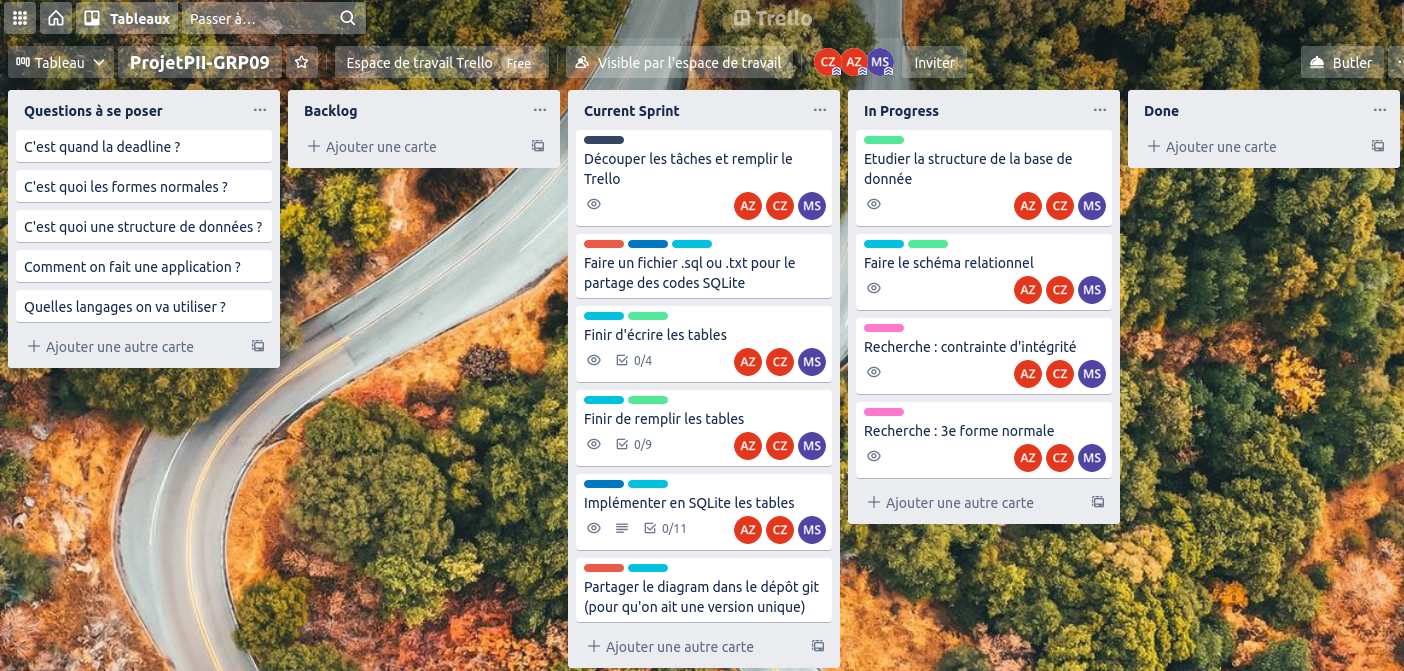
\includegraphics[scale = 0.37]{Images/Gestion de Projet/Trello/Trello_11042021.png}
            \caption{L'organisation du Trello le 11 avril 2021}
            \label{fig:Trello11042021}
        \end{figure}
        \begin{figure}[!h]
            \centering
            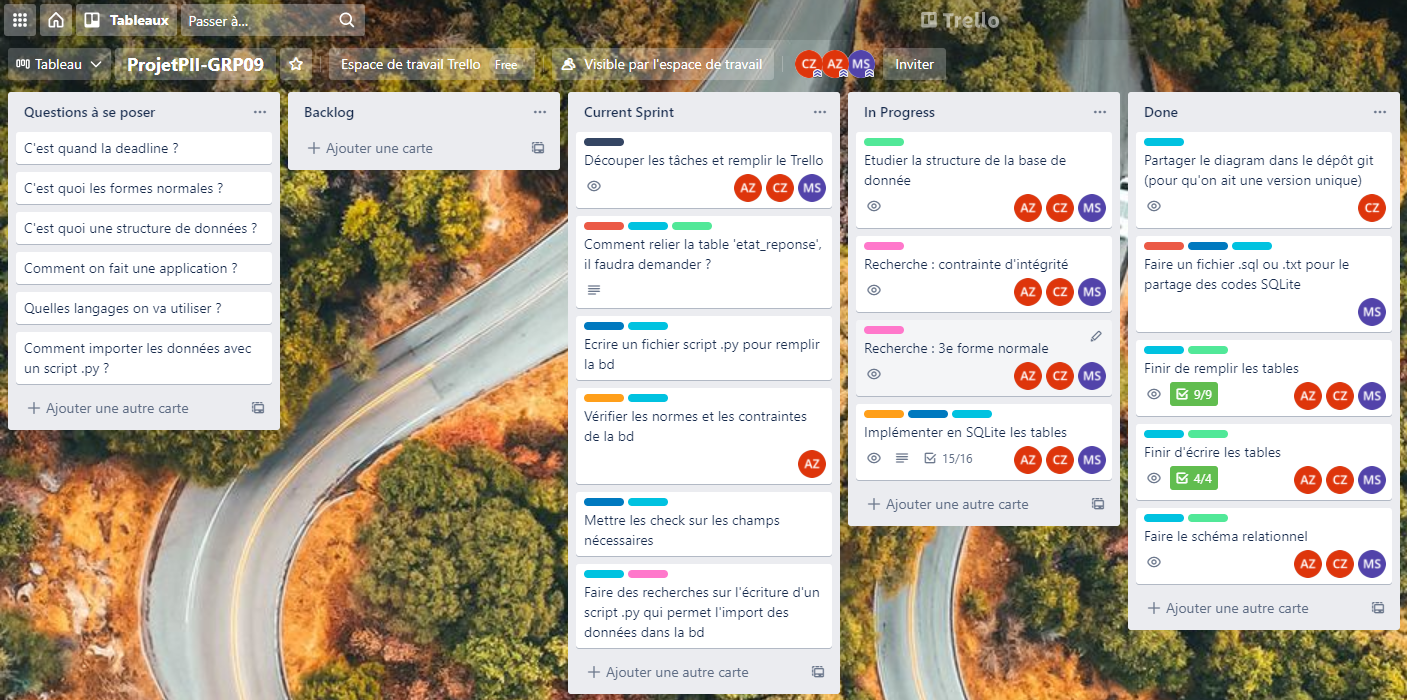
\includegraphics[scale = 0.37]{Images/Gestion de Projet/Trello/Trello_25042021.png}
            \caption{L'organisation du Trello le 25 avril 2021}
        \label{fig:Trello25042021}
        \end{figure}
\newpage
        \begin{figure}[!h]
            \centering
            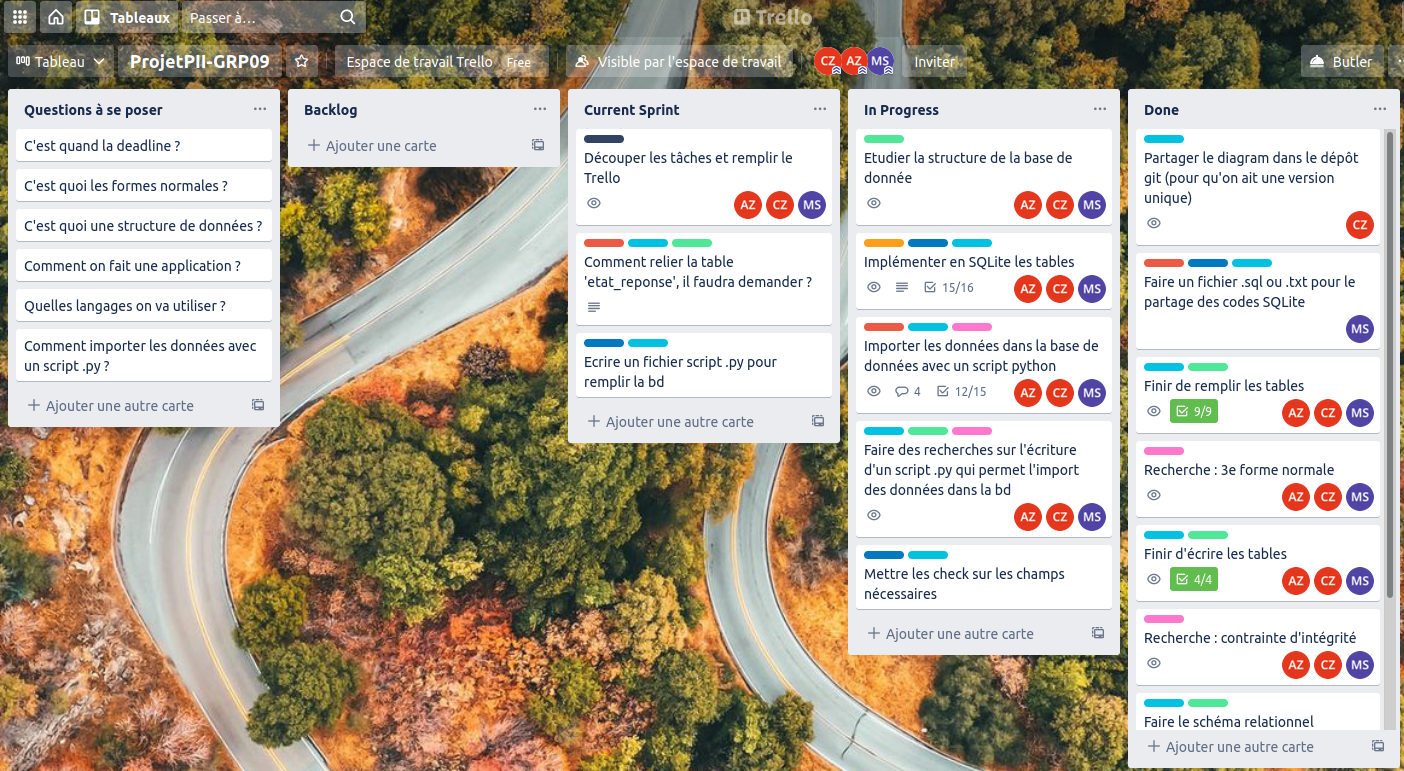
\includegraphics[scale = 0.37]{Images/Gestion de Projet/Trello/Trello_12052021.png}
            \caption{L'organisation du Trello le 12 mai 2021}
            \label{fig:Trello12052021}
        \end{figure}
        %\newpage
        \begin{figure}[!h]
            \centering
            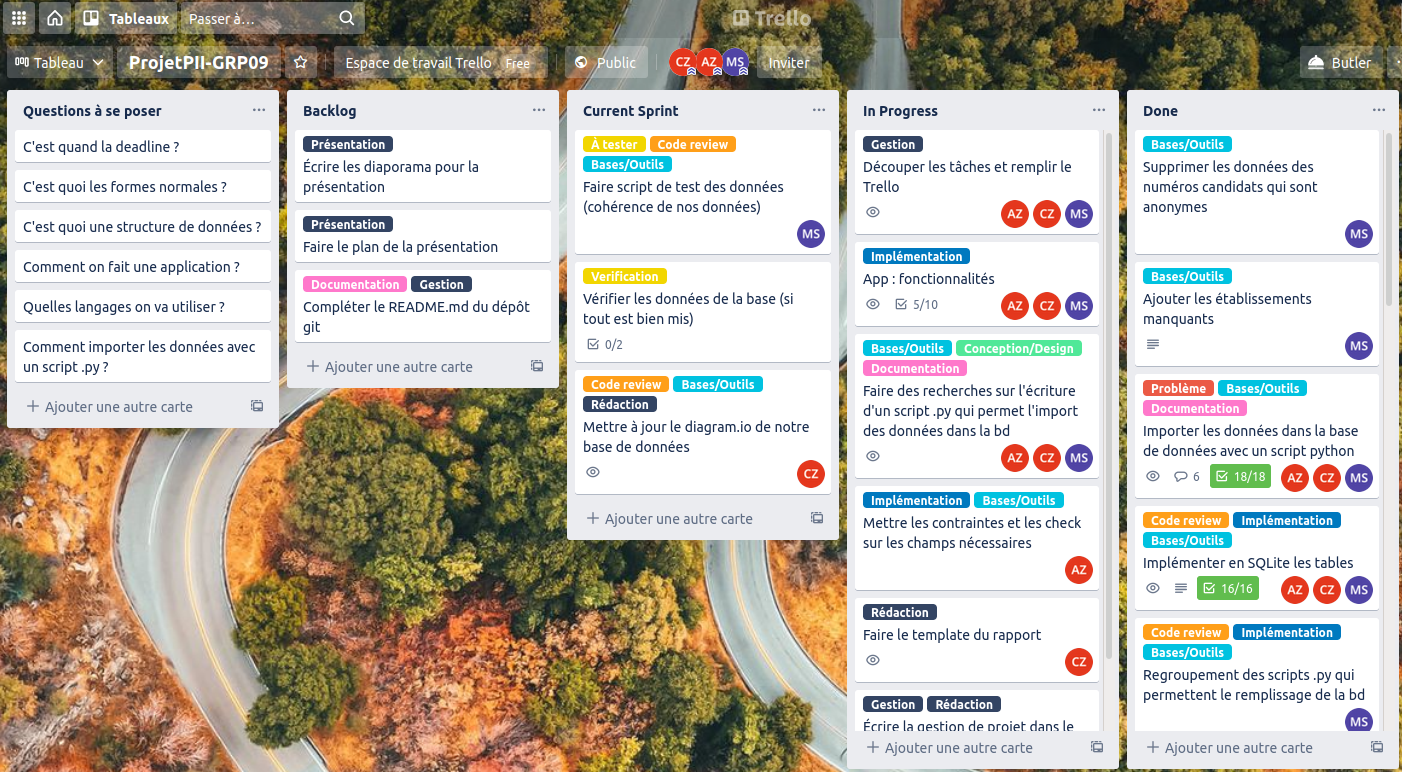
\includegraphics[scale = 0.37]{Images/Gestion de Projet/Trello/Trello_02062021.png}
            \caption{L'organisation du Trello le 2 juin 2021}
            \label{fig:Trello02062021}
        \end{figure}
\newpage
        \begin{figure}[!h]
            \centering
            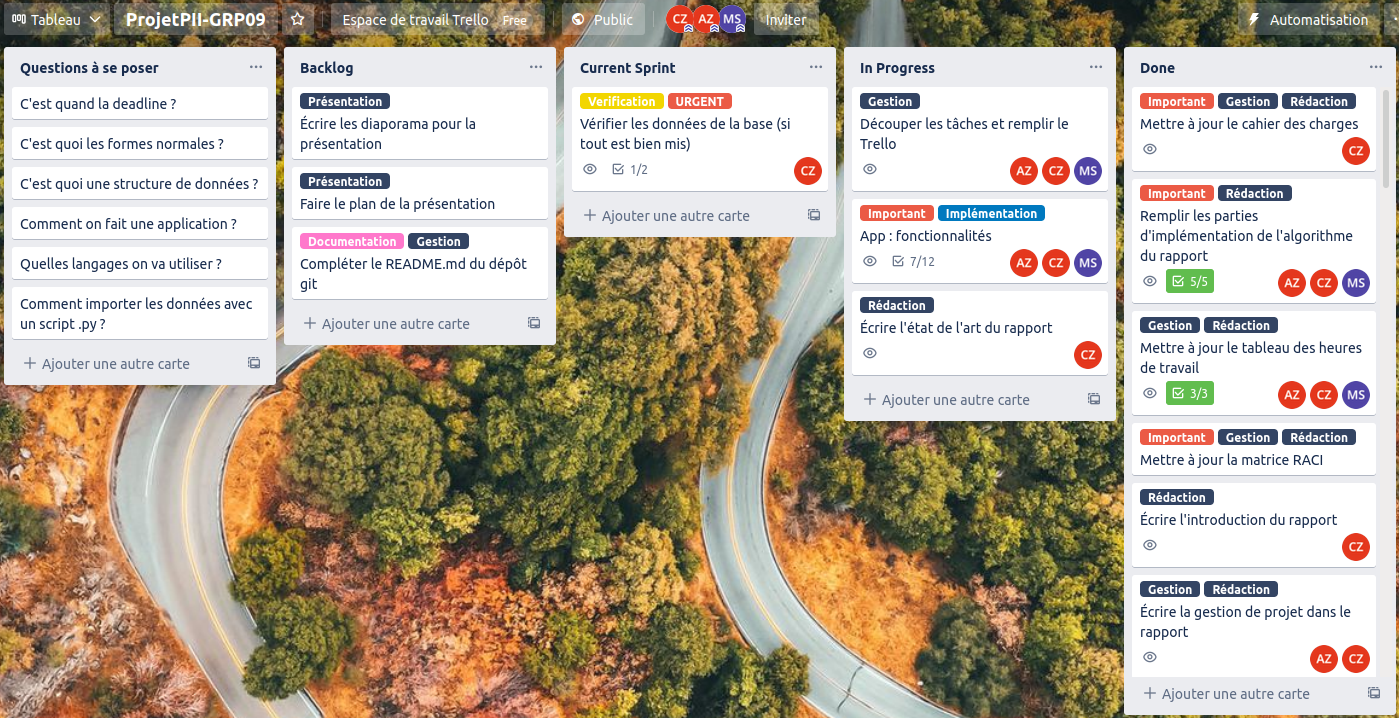
\includegraphics[scale = 0.37]{Images/Gestion de Projet/Trello/Trello_11062021.png}
            \caption{L'organisation du Trello le 11 juin 2021}
            \label{fig:Trello11062021}
        \end{figure}

\newpage

\subsection*{Comptes rendus de réunions}
    \addcontentsline{toc}{subsection}{Comptes rendus de réunions}
    % \documentclass[12pt]{article}
% \usepackage{natbib}
% \usepackage[french]{babel}
% \usepackage[utf8]{inputenc}
% \usepackage[T1]{fontenc}
% \usepackage{tikz}
% \usepackage{amsmath}
% \usepackage{graphics}
% \usepackage{graphicx}
% \usepackage{url}
% \usepackage{psfrag}
% \usepackage{fancyhdr}
% \usepackage{vmargin}
% \usepackage[backend=biber]{biblatex}
% \usepackage{csquotes}
% \usepackage[hidelinks]{hyperref}
% \usepackage{enumitem}

% \pagestyle{fancy}


% \begin{document}
\subsubsection*{\large{Réunion d'équipe du 3 avril 2021}}
    \addcontentsline{toc}{subsubsection}{Réunion d'équipe du 3 avril 2021}
\begin{center}
\begin{tabular}{| l | l || c | c |}
    \hline
    Membres présents & Membres absents & Durée & Lieu \\
    \hline
    Maël SAILLOT & & & \\ Céline ZHANG & & 1h45 & Discord \\ Ahmed ZIANI & & & \\
    \hline
\end{tabular}
\end{center}

\subsubsection*{Ordre du jour}
\begin{enumerate}
    \item Mise à niveau générale sur les connaissances du sujet
    \item Organisation du projet
    \item Sélection des outils nécessaires au projet
    \item Mise en place de la gestion de projet
    \item Planification des prochaines réunions
\end{enumerate}

\subsubsection*{Mise à niveau générale sur les connaissances du sujet}
Nous avons mis en commun nos connaissances concernant le sujet, partagé nos documentations, et expliqué les notions ambigües. Ceci s'est suivi d'une présentation de nos préférences, de nos points forts et points faibles respectives.

\subsubsection*{Organisation du projet}
Nous avons parlé du sens de déroulement général du projet (quand faire les documentations, dans les premières lignes, quand aborder les parties, quand commencer la rédaction du rapport, etc.). Nous avons discuté d'une gestion de projet (les stratégies, les rôles, voir le tableau~\ref{tab:roles}, les facilités, les difficultés par la matrice de SWOT, voir figure~\ref{tab:swot}). Nous adoptons la gestion SCRUM, qui utilise la méthode du \textsl{sprint}\footnotemark \ pour réaliser les travaux.

    \begin{table}[!h]
    \begin{center}
        \begin{tabular}{|l|l|}
        \hline
            Membre de l'équipe 9 & Rôles ou charges \\
        \hline
        \hline
            Céline ZHANG & leader \\
        \hline
            Ahmed ZIANI & reviewer \\
        \hline
            Maël SAILLOT & responsable du git \\
        \hline
        \end{tabular}\\
        %\includegraphics[scale = 0.45]{Images/Gestion de Projet/Matrice_swot.png}
    \end{center}
    %\caption{Tableau des rôles}
    %\label{tab:roles}
    \end{table}

\paragraph{Céline ZHANG} se chargera de vérifier les tâches, les objectifs, de planifier les réunions et d'écrire les compte-rendus de réunions d'équipe.
\paragraph{Ahmed ZIANI} se chargera de revoir nos lignes de code (code review), de vérifier la cohérence et les tests.
\paragraph{Maël SAILLOT} s'occupera de gérer le dépôt git de l'équipe, de gérer les erreurs dû à des conflits.

\footnotetext{Méthode d'organisation de travail d'équipe qui consiste à se fixer des tâches pour un cycle (1 à 2 semaines) et de les finir avant la fin de celle-ci.}

\subsubsection*{Sélection des outils nécessaires au projet}
La présentation des outils utilisables et les outils nécessaires est primordiale pour commencer à travailler. Nous avons donc présenté les outils à disposition (\textsf{gitlab}, \textsf{Discord}, \textsf{SQLite}, \textsf{Overleaf}, \textsf{dbdiagram.io}, \textsl{C}, \textsf{Java}, \textsf{Python}, \textsf{html}).

\subsubsection*{Mise en place de la gestion de projet}
Nous avons choisi d'utiliser le tableau de bord Trello\footnotemark qui va nous permettre de mettre le cahier de charge en tâches nécessaires à la réalisation du livrable final. Ceci nous permet aussi de surveiller l'avancement de chacun sur ses tâches. Nous avons commencé par créer le Trello et y mettre des tâches.
\footnotetext{Outil qui nous permet de planifier en ligne des activités.\ref{fig:exTrello02062021}}

\subsubsection*{Planification des prochaines réunions}
Nous décidons de faire en général une réunion par semaine (flexible suivant les disponibilités), qui sera tous les dimanches à 17h00 sur Discord, bien sûr il peut y avoir des stand-up-meeting pour régler les soucis ou prendre des nouvelles (le tableau Trello permet aussi de laisser des messages pour indiquer les problèmes et demander de l'aide).

\paragraph{\emph{TO-DO LIST}}
\begin{itemize}
    \item Se documenter sur première partie du sujet concernant les notions de 3e forme normale, les contraintes d'intégrités
    \item Réfléchir à la structure de la base de données
    \item Faire un schéma liant les tables
\end{itemize}

\emph{Prochaine réunion : 06/04/2021}\\

% \end{document}
    \newpage
    % \documentclass[12pt]{article}
% \usepackage[french]{babel}
% \usepackage{natbib}
% \usepackage[utf8]{inputenc}
% \usepackage[T1]{fontenc}
% \usepackage{tikz}
% \usepackage{amsmath}
% \usepackage{graphics}
% \usepackage{graphicx}
% \usepackage{url}
% \usepackage{psfrag}
% \usepackage{fancyhdr}
% \usepackage{vmargin}
% \usepackage[backend=biber]{biblatex}
% \usepackage{csquotes}
% \usepackage[hidelinks]{hyperref}
% \usepackage{enumitem}

% \pagestyle{fancy}


% \begin{document}
\subsubsection*{\large{Réunion d'équipe du 6 avril 2021}}
    \addcontentsline{toc}{subsubsection}{Réunion d'équipe du 6 avril 2021}
\begin{center}
\begin{tabular}{| l | l || c | c |}
    \hline
    Membres présents & Membres absents & Durée & Lieu \\
    \hline
    Maël SAILLOT & & & \\ Céline ZHANG & & 1h30 & Telecom Nancy \\ Ahmed ZIANI & & & \\
    \hline
\end{tabular}
\end{center}

\subsubsection*{Ordre du jour}
\begin{enumerate}
    \item Avancement des tâches
    \item Mise en commun des propositions
    \item Optimisation des solutions proposées
    \item Choix des prochaines tables
\end{enumerate}

\subsubsection*{Avancement des tâches}
Les membres sont venus avec leur schéma d'une structures des données. Nous avons pris connaissance de chacun de ces schémas qui étaient globlalement similaires.

\subsubsection*{Mise en commun des propositions}
Nous avons produit un schéma pour l'implémentation du diagram sur une interface graphique \textsf{dbdiagram.io}.

\subsubsection*{Optimisation des solutions proposées}
En prenant en compte les contraintes d'intégrités et en respectant les règles de la 3e forme normale, nous avons choisi de mettre les principales informations de l'inscrit dans une table \texttt{candidat} (comme civilité, nom, prénom, date et lieu de naissance, coordonnées, rang, classe, filière concours, etc.) et certainement dans une deuxième table, les options du candidat. De plus des tables moins grandes ont été faites, comme les tables \texttt{etablissement}, \texttt{voeux}, \texttt{classement}, \texttt{notes}, \texttt{epreuve}, etc. Le numéro du candidat sera une clé primaire, et servira de foreign key pour certaines des tables suivantes.

\subsubsection*{Choix des prochaines tables}
Nous allons sûrement faire une table \texttt{autres\_info}, \texttt{pays}, \texttt{concours}, etc. le nécessaire pour compléter la base de données.

\subsubsection*{Planification des prochaines tâches}
L'équipe devra écrire ces tables sur \textsf{dbdiagram.io}, compléter les champs manquants, et ajouter éventuellement les tables manquantes ; mettre sur Trello les tâches.


\paragraph{\emph{TO-DO LIST}}
\begin{itemize}
    \item Écrire les tables sur \textsf{dbdiagram.io}
    \item Compléter la structure de bases de données (les tables et les champs manquants, etc.)
    \item Mettre les tâches sur le Trello
\end{itemize}

\emph{Prochaine réunion : 11/04/2021}\\

% \end{document}
    \newpage
    % \documentclass[12pt]{article}
% \usepackage[french]{babel}
% \usepackage{natbib}
% \usepackage[utf8]{inputenc}
% \usepackage[T1]{fontenc}
% \usepackage{tikz}
% \usepackage{amsmath}
% \usepackage{graphics}
% \usepackage{graphicx}
% \usepackage{url}
% \usepackage{psfrag}
% \usepackage{fancyhdr}
% \usepackage{vmargin}
% \usepackage[backend=biber]{biblatex}
% \usepackage{csquotes}
% \usepackage[hidelinks]{hyperref}
% \usepackage{enumitem}

% \pagestyle{fancy}


% \begin{document}
\subsubsection*{\large{Réunion d'équipe du 11 avril 2021}}
    \addcontentsline{toc}{subsubsection}{Réunion d'équipe du 11 avril 2021}
\begin{center}
\begin{tabular}{| l | l || c | c |}
    \hline
    Membres présents & Membres absents & Durée & Lieu \\
    \hline
    Maël SAILLOT & & & \\ Céline ZHANG & & 1h & Discord \\ Ahmed ZIANI & & & \\
    \hline
\end{tabular}
\end{center}

\subsubsection*{Ordre du jour}
\begin{enumerate}
    \item Avancement des tâches
    \item Discussion générale des avis sur la structure actuelle
    \item Optimisation des solutions proposées
    \item Prochaines tâches
\end{enumerate}

\subsubsection*{Avancement des tâches}
\paragraph{Maël SAILLOT} a écrit dans le \textsf{dbdiagram.io} la première version de la structure de la base de données et l'a partagé aux autres membres.
\paragraph{Céline ZHANG} a complété une partie des champs manquants dans les tables et ajouté une partie des tables manquantes.
\paragraph{Ahmed ZIANI} a proposé une solution en faisant des tables \texttt{admissible\_XX}, \texttt{admis\_XX} pour chaque filière.

\subsubsection*{Discussion générale des avis sur la structure actuelle}
La proposition des tables \texttt{admissible\_XX}, \texttt{admis\_XX} pour chaque filière a finalement été rejeté, puisqu'il y aurait redonnance des données, par ailleurs, il se trouvait déjà dans le champ \texttt{type} (qui n'avait pas été explicité, d'où le malentendu avec les tables \texttt{admissible\_XX}, \texttt{admis\_XX}).

\subsubsection*{Optimisation des solutions proposées}
Nous avons vérifié les relations entre les tables, et corrigé quelques imprecision des champs. Nous avons rajouté des notes et restrictions pour certains champs. Après discussion, nous avons choisi de mettre une partie des info candidat dans candidat, et une autre partie certainement dans une autre table, elles seront liées par une relation 1 1.

\subsubsection*{Prochaines tâches}
L'équipe devra compléter les tables, et écrire les tables restantes sur \textsf{dbdiagram.io}. Ensuite, chaque membre fera 3 à 4 tables en SQLite, et mettra leur code sur un fichier \textsf{.sql} (ou \textsf{.txt}) partagé sur le \textsf{git}. Chacun sera libre de choisir les tables qu'il fera, mais il devra indiquer sur le Trello son choix et \textsl{push} son travail pour tenir au courant les autres membres. Une description détaillée de ce qui est à faire se trouve sur le Discord de l'équipe, dans le canal \textsl{\#todo}.


\paragraph{\emph{TO-DO LIST}}
\begin{itemize}
    \item Finir de mettre les tables manquantes (voir le canal \textsl{\#todo} sur le Discord de l'équipe)
    \item Finir de remplir les champs des tables (voir le canal \textsl{\#todo} sur Discord)
    \item Implémenter ces tables en SQLite et partager les codes sur le dépôt \texttt{git}
    \item Mettre à jour le Trello
    
\end{itemize}

\emph{Prochaine réunion : 25/04/2021}\\

% \end{document}
    \newpage
    % \documentclass[12pt]{article}
% \usepackage[french]{babel}
% \usepackage{natbib}
% \usepackage[utf8]{inputenc}
% \usepackage[T1]{fontenc}
% \usepackage{tikz}
% \usepackage{amsmath}
% \usepackage{graphics}
% \usepackage{graphicx}
% \usepackage{url}
% \usepackage{psfrag}
% \usepackage{fancyhdr}
% \usepackage{vmargin}
% \usepackage[backend=biber]{biblatex}
% \usepackage{csquotes}
% \usepackage[hidelinks]{hyperref}
% \usepackage{enumitem}

% \pagestyle{fancy}


% \begin{document}
\subsubsection*{\large{Réunion d'équipe du 25 avril 2021}}
    \addcontentsline{toc}{subsubsection}{Réunion d'équipe du 25 avril 2021}
\begin{center}
\begin{tabular}{| l | l || c | c |}
    \hline
    Membres présents & Membres absents & Durée & Lieu \\
    \hline
    Maël SAILLOT & & & \\ Céline ZHANG & & 1h40 & Discord \\ Ahmed ZIANI & & & \\
    \hline
\end{tabular}
\end{center}

\subsubsection*{Ordre du jour}
\begin{enumerate}
    \item Avancement des tâches
    \item Discussion générale et amélioration de la structure actuelle
    \item Prochaines tâches
\end{enumerate}

\subsubsection*{Avancement des tâches}
\paragraph{Maël SAILLOT} a ajouté les tables, les champs manquants, a créé les fichiers \textsf{createdb.sql} et \textsf{schemadb.txt} pour le partage.
\paragraph{Céline ZHANG} a revu les codes du schéma de \textsf{dbdiagram.io}, a commencé à remplir le fichier \textsf{createdb.sql}.
\paragraph{Ahmed ZIANI} a relu les travaux de l'équipe.

\subsubsection*{Discussion générale et amélioration de la structure actuelle}
Nous avons relu chaque ligne de schéma, nous avons fixé les contraintes nécessaires sur certains champs, et corrigé les erreurs. Les codes postaux doivent être en \textsf{TEXT} car les adresses étrangères ont des lettres dans leur code postal, idem pour les numéros particulier comme \textsf{+33(0)}.

\subsubsection*{Prochaines tâches}
L'équipe devra compléter le fichier \textsf{createdb.sql}, ajouter les contraintes, vérifier le respect des formes normalisés et les contraintes (\textsl{review}), et se renseigner sur l'écriture d'un script en \textsf{Python} qui permettra de remplir la base de données de manière automatique.


\paragraph{\emph{TO-DO LIST}}
\begin{itemize}
    \item Remplir le fichier \textsf{createdb.sql} et tester l'exécution de celui-ci
    \item Ajouter les \textsf{CHECK} nécessaires (voir le canal \textsl{\#todo} sur Discord)
    \item Partager fichier \textsf{.py} sur le dépôt \texttt{git}
    \item Se documenter sur l'écriture du script en \textsf{.py}
    \item Écrire un exemple de fonction dans le script pour l'import des données
    
\end{itemize}

\emph{Prochaine réunion : 29/04/2021}\\

% \end{document}
    \newpage
    % \documentclass[12pt]{article}
% \usepackage[french]{babel}
% \usepackage{natbib}
% \usepackage[utf8]{inputenc}
% \usepackage[T1]{fontenc}
% \usepackage{tikz}
% \usepackage{amsmath}
% \usepackage{graphics}
% \usepackage{graphicx}
% \usepackage{url}
% \usepackage{psfrag}
% \usepackage{fancyhdr}
% \usepackage{vmargin}
% \usepackage[backend=biber]{biblatex}
% \usepackage{csquotes}
% \usepackage[hidelinks]{hyperref}
% \usepackage{enumitem}

% \pagestyle{fancy}


% \begin{document}
\subsubsection*{\large{Réunion d'équipe du 29 avril 2021}}
    \addcontentsline{toc}{subsubsection}{Réunion d'équipe du 29 avril 2021}
\begin{center}
\begin{tabular}{| l | l || c | c |}
    \hline
    Membres présents & Membres absents & Durée & Lieu \\
    \hline
    Maël SAILLOT & & & \\ Céline ZHANG & & 1h10 & Discord \\ Ahmed ZIANI & & & \\
    \hline
\end{tabular}
\end{center}

\subsubsection*{Ordre du jour}
\begin{enumerate}
    \item Avancement des tâches
    \item Discussion générale et amélioration du travail actuel
    \item Prochaines tâches
\end{enumerate}

\subsubsection*{Avancement des tâches}
Glogalement chaque membre a fait ses recherches pour trouver un moyen de remplir la base de données à partir des fichiers \textsf{.xlsx} donnés.
\paragraph{Maël SAILLOT} a fait un exemple de script pour le remplissage de la table des \texttt{etat\_reponse} en utilisant la bibliothèque \texttt{openpyxl} et a fait deux versions, l'une utilisant \textsf{click}, l'autre sans.
\paragraph{Céline ZHANG} a fait un exemple de script pour le remplissage à partir du fichier \textsf{Inscription.xlsx} en utilisant la bibliothèque \texttt{pandas}.
\paragraph{Ahmed ZIANI} a fait un exemple de script pour le remplissage de la table des \texttt{etat\_reponse} en utilisant la bibliothèque \texttt{openpyxl} et a essayé avec \texttt{pandas} aussi.

\subsubsection*{Discussion générale et amélioration du travail actuel}
Nous avons relu le fichier \textsf{createdb.sql}, nous constatons qu'il fallait ajouter des \textsf{CHECK}. Nous avons choisi d'utiliser principalement la bibliothèque \texttt{pandas} bien qu'elle est plus coûteuse en mémoire par rapport à \texttt{openpyxl} (elle permet la lecture des titre de colonne), nous utiliserons également \texttt{openpyxl} pour d'autres cas.

\subsubsection*{Prochaines tâches}
L'équipe devra écrire les algorithmes de remplissage des tables de la base de données en faisant en priorité les tables qui ont le moins de dépendances par rapport aux autres tables. Il faudra vérifier les contraintes des champs et réfléchir sur les ATS.


\paragraph{\emph{TO-DO LIST}}
\begin{itemize}
    \item Écrire les algorithmes de remplissage selon les priorités et la \textsl{checklist} sur Trello
    \item Vérifier les contraintes et les tables
    \item Réfléchir au cas des ATS
    
\end{itemize}

\emph{Prochaine réunion : 03/05/2021}\\

% \end{document}
    \newpage
    % \documentclass[12pt]{article}
% \usepackage[french]{babel}
% \usepackage{natbib}
% \usepackage[utf8]{inputenc}
% \usepackage[T1]{fontenc}
% \usepackage{tikz}
% \usepackage{amsmath}
% \usepackage{graphics}
% \usepackage{graphicx}
% \usepackage{url}
% \usepackage{psfrag}
% \usepackage{fancyhdr}
% \usepackage{vmargin}
% \usepackage[backend=biber]{biblatex}
% \usepackage{csquotes}
% \usepackage[hidelinks]{hyperref}
% \usepackage{enumitem}

% \pagestyle{fancy}


% \begin{document}
\subsubsection*{\large{Réunion d'équipe du 3 mai 2021}}
    \addcontentsline{toc}{subsubsection}{Réunion d'équipe du 3 mai 2021}
\begin{center}
\begin{tabular}{| l | l || c | c |}
    \hline
    Membres présents & Membres absents & Durée & Lieu \\
    \hline
    Maël SAILLOT & & & \\ Céline ZHANG & & 1h & Discord \\ Ahmed ZIANI & & & \\
    \hline
\end{tabular}
\end{center}

\subsubsection*{Ordre du jour}
\begin{enumerate}
    \item Avancement des tâches
    \item Discussion générale et amélioration du travail actuel
    \item Prochaines tâches
\end{enumerate}

\subsubsection*{Avancement des tâches}
\paragraph{Maël SAILLOT} a rempli la table \texttt{etat\_reponse}.
\paragraph{Céline ZHANG} a rempli les tables \texttt{etat\_dossier}, \texttt{concours}, \texttt{autres\_prenoms}, \texttt{serie\_bac}, \texttt{ep\_option}.
\paragraph{Ahmed ZIANI} a rempli les tables \texttt{ecole}, \texttt{etablissement}, \texttt{pays}, \texttt{csp\_parent}.

\subsubsection*{Discussion générale et amélioration du travail actuel}
Pour le remplissage de \texttt{epreuve}, il a fallu un dictionnaire. Nous avons choisi de réutiliser les codes proposées par les fichiers comme clé primaire et nous avons ajouté certains code pour les champs qui n'en possédaient pas. Les codes ajoutés commence à partir de 9000, par exemple 9898 pour la \texttt{bonification\_ecrit}. Nous avons remarqué que les champs \texttt{etat\_classes} et \texttt{type\_admissible} n'étaient pas dans nos tables de la base de données, il a fallu les ajouter. Certains champs manquaient des \texttt{NOT NULL}, il faut les ajouter. Concernant les ATS, certains candidats n'avaient pas de données pour certains champs, nous avons choisi d'ignorer les candidats anonymes (qui n'ont ni nom, ni prénom).

\subsubsection*{Prochaines tâches}
L'équipe devra finir d'écrire les algorithmes de remplissage des tables de la base de données (en faisant attention aux nouveaux champs ajoutés), elle devra ajouter les \texttt{NOT NULL} nécessaire, et commencer le remplissage des candidats d'ATS.


\paragraph{\emph{TO-DO LIST}}
\begin{itemize}
    \item Finir le remplissage des tables de la \textsl{checklits} sur Trello
    \item Ajouter les \texttt{NOT NULL} et vérifier les contraintes
    \item Commencer le remplissage pour les ATS
    
\end{itemize}

\emph{Prochaine réunion : 14/05/2021}\\

% \end{document}
    \newpage
    % \documentclass[12pt]{article}
% \usepackage[french]{babel}
% \usepackage{natbib}
% \usepackage[utf8]{inputenc}
% \usepackage[T1]{fontenc}
% \usepackage{tikz}
% \usepackage{amsmath}
% \usepackage{graphics}
% \usepackage{graphicx}
% \usepackage{url}
% \usepackage{psfrag}
% \usepackage{fancyhdr}
% \usepackage{vmargin}
% \usepackage[backend=biber]{biblatex}
% \usepackage{csquotes}
% \usepackage[hidelinks]{hyperref}
% \usepackage{enumitem}

% \pagestyle{fancy}


% \begin{document}
\subsubsection*{\large{Réunion d'équipe du 14 mai 2021}}
    \addcontentsline{toc}{subsubsection}{Réunion d'équipe du 14 mai 2021}
\begin{center}
\begin{tabular}{| l | l || c | c |}
    \hline
    Membres présents & Membres absents & Durée & Lieu \\
    \hline
    Maël SAILLOT & & & \\ Céline ZHANG & & 40min & Discord \\ Ahmed ZIANI & & & \\
    \hline
\end{tabular}
\end{center}

\subsubsection*{Ordre du jour}
\begin{enumerate}
    \item Avancement des tâches
    \item Discussion générale et amélioration du travail actuel
    \item Prochaines tâches
\end{enumerate}

\subsubsection*{Avancement des tâches}
\paragraph{Maël SAILLOT} a vérifié les contraintes et le dépôt \textsf{git}.
\paragraph{Céline ZHANG} a rempli les tables \texttt{epreuvre}, \texttt{notes}, \texttt{classement}, a écrit les dictionnaires des épreuves et des classements nécessaire à l'algorithme de remplissage.
\paragraph{Ahmed ZIANI} a rempli la table \texttt{voeux}.

\subsubsection*{Discussion générale et amélioration du travail actuel}
La plupart des tables ont été remplies, cependant les ATS n'ont pas été ajoutés, il manque également la remplissage de la table \texttt{candidat}. Pour l'instant chacun a son \textsl{script}, les tests ont été fait manuellement lors de l'import des données dans les tables de la base de données. Il faut maintenant les regrouper dans un \textsl{script} et optimiser le code de chacun. De plus, pour vérifier la cohérence des données, il est nécessaire de faire un \textsl{script} de test.

\subsubsection*{Prochaines tâches}
L'équipe devra remplir la table \texttt{candidat} avec vérification manuelle, puis faire un \textsl{script} pour vérifier la cohérence des données importer avec la bd et les fichiers. Il faudra écrire les algorithmes de remplissage pour les ATS, et regrouper tous les codes dans un \textsl{script} qui rempli en une fois toute la base de données.


\paragraph{\emph{TO-DO LIST}}
\begin{itemize}
    \item Remplir la table \texttt{candidat}
    \item Ajouter les données des candidats ATS
    \item Faire un \textsl{script} qui regroupe tous les codes
    \item Commencer un \textsl{script} de test
    
\end{itemize}

\emph{Prochaine réunion : 24/05/2021}\\

% \end{document}
    \newpage
    % \documentclass[12pt]{article}
% \usepackage[french]{babel}
% \usepackage{natbib}
% \usepackage[utf8]{inputenc}
% \usepackage[T1]{fontenc}
% \usepackage{tikz}
% \usepackage{amsmath}
% \usepackage{graphics}
% \usepackage{graphicx}
% \usepackage{url}
% \usepackage{psfrag}
% \usepackage{fancyhdr}
% \usepackage{vmargin}
% \usepackage[backend=biber]{biblatex}
% \usepackage{csquotes}
% \usepackage[hidelinks]{hyperref}
% \usepackage{enumitem}

% \pagestyle{fancy}


% \begin{document}
\subsubsection*{\large{Réunion d'équipe du 24 mai 2021}}
    \addcontentsline{toc}{subsubsection}{Réunion d'équipe du 24 mai 2021}
\begin{center}
\begin{tabular}{| l | l || c | c |}
    \hline
    Membres présents & Membres absents & Durée & Lieu \\
    \hline
    Maël SAILLOT & & & \\ Céline ZHANG & & 1h30 & Discord \\ Ahmed ZIANI & & & \\
    \hline
\end{tabular}
\end{center}

\subsubsection*{Ordre du jour}
\begin{enumerate}
    \item Avancement des tâches
    \item Discussion générale et amélioration du travail actuel
    \item Prochaines tâches
\end{enumerate}

\subsubsection*{Avancement des tâches}
\paragraph{Maël SAILLOT} a rempli la table \texttt{candidat}, a ajouté les ATS.
\paragraph{Céline ZHANG} a corrigé les contraintes qui se trouvaient dans \texttt{createdb.sql}.
\paragraph{Ahmed ZIANI} a vérifié et a ajouté les contraintes nécessaires.

\subsubsection*{Discussion générale et amélioration du travail actuel}
En remplissant les ATS et la table \texttt{candidat}, nous remarquons que certains établissements ne se trouvent pas dans le fichier \texttt{listeEtablissements.xlsx} alors qu'ils se trouvent dans les informations des candidats. De plus, certains candidats avaient des notes ou un classement, mais ne se trouvaient pas dans la table \texttt{candidat}, ils ne sont pas dans le fichier \texttt{Inscription.xlsx}. Les TSI dans le fichier \texttt{Ecrit\_TSI.xlsx} n'ont pas de rang. L'équipe a choisi de partir sur une application web écrit en \textsf{Python} en utilisant le module \textsf{Flask}.

\subsubsection*{Prochaines tâches}
L'équipe devra supprimer toutes les données engendrants des incohérences (notamment ceux des candidats anonymes). Elle devra également ajouter les établissements manquants. Une vérification de l'ensemble des données sera nécessaire pour être sûr que rien n'a été négligé.


\paragraph{\emph{TO-DO LIST}}
\begin{itemize}
    \item Supprimer les candidats anonymes
    \item Ajouter les établissements manquants
    \item Regrouper les scripts en un seul script optimisé
    \item Faire le script de test pour vérifier la cohérence des données
    \item Commencer l'écriture de l'application web
    
\end{itemize}

\emph{Prochaine réunion : 04/06/2021}\\

% \end{document}
    \newpage
    % \documentclass[12pt]{article}
% \usepackage[french]{babel}
% \usepackage{natbib}
% \usepackage[utf8]{inputenc}
% \usepackage[T1]{fontenc}
% \usepackage{tikz}
% \usepackage{amsmath}
% \usepackage{graphics}
% \usepackage{graphicx}
% \usepackage{url}
% \usepackage{psfrag}
% \usepackage{fancyhdr}
% \usepackage{vmargin}
% \usepackage[backend=biber]{biblatex}
% \usepackage{csquotes}
% \usepackage[hidelinks]{hyperref}
% \usepackage{enumitem}

% \pagestyle{fancy}


% \begin{document}
\subsubsection*{\large{Réunion d'équipe du 4 juin 2021}}
    \addcontentsline{toc}{subsubsection}{Réunion d'équipe du 4 juin 2021}
\begin{center}
\begin{tabular}{| l | l || c | c |}
    \hline
    Membres présents & Membres absents & Durée & Lieu \\
    \hline
    Maël SAILLOT & & & \\ Céline ZHANG & & 1h30 & Discord \\ Ahmed ZIANI & & & \\
    \hline
\end{tabular}
\end{center}

\subsubsection*{Ordre du jour}
\begin{enumerate}
    \item Avancement des tâches
    \item Discussion générale et amélioration du travail actuel
    \item Prochaines tâches
\end{enumerate}

\subsubsection*{Avancement des tâches}
\paragraph{Maël SAILLOT} a regroupé les scripts de remplissage pour en faire un seul script optimisé, a commencé le script de test de cohérence entre les fichiers et a mis à jour le schéma de la base de données.
\paragraph{Céline ZHANG} a fait le template du rapport, a fini l'écriture de l'introduction et de la gestion de projet, a ajouté les comptes rendus et les mentions légales, ainsi que d'autres annexes.
\paragraph{Ahmed ZIANI} a fait la matrice \textsf{SWOT}, \textsf{RACI} et a fait les premières fonctionnalités de l'application de web tels que l'affichage des données d'un candidat, la liste des épreuves, des options, des professions, des classements, des notes, etc.

\subsubsection*{Discussion générale et amélioration du travail actuel}
Il faudra vérifier les fichiers, et penser à faire un script de test de remplissage. Il manque pour l'application les fonctionnalités de mises en stats, d'affichage de graphes ou de cartes et les interactions permettant de rendre l'application plus facile d'utilisation. 

\subsubsection*{Prochaines tâches}
L'équipe devra écrire l'état de l'art, finir le script de test de cohérence, ajouter les fonctionnalités stats, cartographique, les styles et l'interface.


\paragraph{\emph{TO-DO LIST}}
\begin{itemize}
    % \item Finir l'application web
    \item Écrire l'état de l'art
    \item Finir le script de test de cohérence
    \item Ajouter les fonctionnalités stats
    \item Ajouter du style et une interface
    \item Ajouter la cartographie et éventuellement des graphes
    % \item Écrire l'explication des algorithmes
    % \item Ajouter les commentaires sur le code
    % \item Mettre à jour le \textsf{README.md}
    % \item Réfléchir à la présentation
    
\end{itemize}

%\emph{Prochaine réunion : 09/06/2021}\\

% \end{document}
    \newpage


\listoffigures
\listoftables

\newpage

\addcontentsline{toc}{section}{Bibliographie}
\bibliographystyle{unsrt}
\bibliography{bibsource}


\end{document}